%%%%%%%%%%%%%%%%%%%%%%%%%%%%%%%%%%%%%%%%%%%%%%%%%%%%%%%%%%%%%%%%%%%%%%%%%%%%
% AGUJournalTemplate.tex: this template file is for articles formatted with LaTeX
%
% This file includes commands and instructions
% given in the order necessary to produce a final output that will
% satisfy AGU requirements, including customized APA reference formatting.
%
% You may copy this file and give it your
% article name, and enter your text.
%
% guidelines and troubleshooting are here: 

%% user added for convenience, can be removed before submission:



%% To submit your paper:
\documentclass[draft]{agujournal2019}
\usepackage{url} %this package should fix any errors with URLs in refs.
\usepackage{lineno}
\usepackage[inline]{trackchanges} %for better track changes. finalnew option will compile document with changes incorporated.
\usepackage{soul}

% MY OWN ADDED PACKAGES TO RENDER UNITS
\usepackage{gensymb}
\usepackage{booktabs}
\usepackage{siunitx}

\linenumbers
%%%%%%%
% As of 2018 we recommend use of the TrackChanges package to mark revisions.
% The trackchanges package adds five new LaTeX commands:
%
%  \note[editor]{The note}
%  \annote[editor]{Text to annotate}{The note}
%  \add[editor]{Text to add}
%  \remove[editor]{Text to remove}
%  \change[editor]{Text to remove}{Text to add}
%
% complete documentation is here: http://trackchanges.sourceforge.net/
%%%%%%%

\draftfalse

%% Enter journal name below.
%% Choose from this list of Journals:
%
% JGR: Atmospheres
% JGR: Biogeosciences
% JGR: Earth Surface
% JGR: Oceans
% JGR: Planets
% JGR: Solid Earth
% JGR: Space Physics
% Global Biogeochemical Cycles
% Geophysical Research Letters
% Paleoceanography and Paleoclimatology
% Radio Science
% Reviews of Geophysics
% Tectonics
% Space Weather
% Water Resources Research
% Geochemistry, Geophysics, Geosystems
% Journal of Advances in Modeling Earth Systems (JAMES)
% Earth's Future
% Earth and Space Science
% Geohealth
%
% ie, \journalname{Water Resources Research}

\journalname{JGR: Biogeosciences}


\begin{document}

%%%%%%%%%%%%%%%%%%%%%%%%%%%%%%%%%%%%%%%%%%%%%%%
%  TITLE
%
% (A title should be specific, informative, and brief. Use
% abbreviations only if they are defined in the abstract. Titles that
% start with general keywords then specific terms are optimized in
% searches)
%
%%%%%%%%%%%%%%%%%%%%%%%%%%%%%%%%%%%%%%%%%%%%%%%

% Example: \title{This is a test title}

\title{Climate-driven phytoplankton community variability in the Cariaco Basin, Venezuela}

%%%%%%%%%%%%%%%%%%%%%%%%%%%%%%%%%%%%%%%%%%%%%%%
%
%  AUTHORS AND AFFILIATIONS
%
%%%%%%%%%%%%%%%%%%%%%%%%%%%%%%%%%%%%%%%%%%%%%%%

% Authors are individuals who have significantly contributed to the
% research and preparation of the article. Group authors are allowed, if
% each author in the group is separately identified in an appendix.)

% List authors by first name or initial followed by last name and
% separated by commas. Use \affil{} to number affiliations, and
% \thanks{} for author notes.
% Additional author notes should be indicated with \thanks{} (for
% example, for current addresses).

% Example: \authors{A. B. Author\affil{1}\thanks{Current address, Antartica}, B. C. Author\affil{2,3}, and D. E.
% Author\affil{3,4}\thanks{Also funded by Monsanto.}}

\authors{Benjamin Post\affil{1,2}, Esteban Acevedo-Trejos\affil{3}, Subhendu Chakraborty\affil{1}, Andrew D. Barton\affil{4}, Agostino Merico\affil{1}}


% \affiliation{1}{First Affiliation}
% \affiliation{2}{Second Affiliation}
% \affiliation{3}{Third Affiliation}
% \affiliation{4}{Fourth Affiliation}

\affiliation{1}{Systems Ecology Group, Leibniz Centre for Tropical Marine Research (ZMT), Bremen, Germany}
\affiliation{2}{School of Science, Constructor University, Bremen, Germany}
\affiliation{3}{Earth Surface Process Modelling, GFZ German Research Centre for Geosciences, Potsdam, Germany}
\affiliation{4}{Scripps Institution of Oceanography and Department of Ecology, Behavior and Evolution, University of California San Diego, La Jolla, CA, United States}
%(repeat as many times as is necessary)


% Corresponding author mailing address and e-mail address:

% (include name and email addresses of the corresponding author.  More
% than one corresponding author is allowed in this LaTeX file and for
% publication; but only one corresponding author is allowed in our
% editorial system.)

% Example: \correspondingauthor{First and Last Name}{email@address.edu}

\correspondingauthor{Benjamin Post}{benjaminpost@aoop.de}



%%%%%%%%%%%%%%%%%%%%%%%%%%%%%%%%%%%%%%%%%%%%%%%
% KEY POINTS
%%%%%%%%%%%%%%%%%%%%%%%%%%%%%%%%%%%%%%%%%%%%%%%
%  List up to three key points (at least one is required)
%  Key Points summarize the main points and conclusions of the article
%  Each must be 140 characters or fewer with no special characters or punctuation and must be complete sentences

% Example:
% \begin{keypoints}
% \item	List up to three key points (at least one is required)
% \item	Key Points summarize the main points and conclusions of the article
% \item	Each must be 140 characters or fewer with no special characters or punctuation and must be complete sentences
% \end{keypoints}

\begin{keypoints}
\item The CARIACO phytoplankton community time series reveals two clusters, separated by a shift from high- to low-upwelling conditions after 2004 and a return to high-upwelling conditions following 2013.
\item No significant differences are observed in diversity metrics between the two clusters, with the exception of a lower turnover and a higher community evenness during low-upwelling conditions.
\item Gradient forest analysis identifies the AMO climate index as the strongest predictor of community change, highlighting the influence of large-scale climatic oscillations on this tropical coastal ecosystem.
\end{keypoints}

%%%%%%%%%%%%%%%%%%%%%%%%%%%%%%%%%%%%%%%%%%%%%%%
%
%  ABSTRACT and PLAIN LANGUAGE SUMMARY
%
% A good Abstract will begin with a short description of the problem
% being addressed, briefly describe the new data or analyses, then
% briefly states the main conclusion(s) and how they are supported and
% uncertainties.

% The Plain Language Summary should be written for a broad audience,
% including journalists and the science-interested public, that will not have 
% a background in your field.
%
% A Plain Language Summary is required in GRL, JGR: Planets, JGR: Biogeosciences,
% JGR: Oceans, G-Cubed, Reviews of Geophysics, and JAMES.
% see http://sharingscience.agu.org/creating-plain-language-summary/)
%
%%%%%%%%%%%%%%%%%%%%%%%%%%%%%%%%%%%%%%%%%%%%%%%

%% \begin{abstract} starts the second page of the manuscript

\begin{abstract}
Phytoplankton communities play a crucial role in oceans' biogeochemical cycles. Climate drives changes in the physical environment that phytoplankton communities experience, thus impacting the productivity and diversity of marine ecosystems. Long-term time series can capture changes in climate and ecosystems, allowing us to untangle the effects on local communities. 
This study aims to describe and investigate the changes in the phytoplankton community of the Cariaco Basin, Venezuela, between 1995 and 2017. Water samples were taken during monthly cruises to determine microscopy cell counts and biogeochemical properties, which we integrated with data from the AMO and MEI v.2 climate indices and ERA5 climate model reanalysis data. 
Using clustering algorithms, we investigate the structure of the community data, revealing two clusters that describe a shift from high- to low-upwelling conditions in 2004, but also show a return to a community and conditions similar to those before the shift in 2014.
However,  community diversity did not follow the same pattern, showing a decrease between 1998 and 2009. To quantify the effect of climate and bottom-up drivers on phytoplankton community changes, we employed a gradient forest analysis and found that a combination of in situ upwelling-related variables (SST and nitrate concentration) and climate indices (AMO and MEI v.2) were the strongest predictors. Our study emphasizes the impact of long-term (decadal) climatic oscillations, such as the AMO, on the phytoplankton community of a tropical coastal ecosystem through modulation of the upwelling system and highlights the capability of ecosystems to recover from the effects of climate change. 

\end{abstract}

%1
\section*{Plain Language Summary}
%Enter your Plain Language Summary here or delete this section.
%Here are instructions on writing a Plain Language Summary: 
%https://www.agu.org/Share-and-Advocate/Share/Community/Plain-language-summary

Microscopic algae drive... (Will write this Summary last, after draft is finalized) 


%%%%%%%%%%%%%%%%%%%%%%%%%%%%%%%%%%%%%%%%%%%%%%%
%                                             %
%  BODY TEXT                                  %
%                                             %
%%%%%%%%%%%%%%%%%%%%%%%%%%%%%%%%%%%%%%%%%%%%%%%

%Comments from Subhi:
    % - first 2 paragraphs, repetetive, put previously known parts into intro, just start from "the problem"
    % - streamline discussion, much shorter!
    % - 


%%% Suggested section heads:
\section{Introduction}
%
% The main text should start with an introduction. Except for short
% manuscripts (such as comments and replies), the text should be divided
% into sections, each with its own heading.

% Headings should be sentence fragments and do not begin with a
% lowercase letter or number. Examples of good headings are:

    % Phytoplankton is important
    Phytoplankton provide the foundation for marine food webs and play a crucial role in biogeochemical processes, including oxygen production and carbon export to the deep ocean \cite{falkowski_biogeochemical_1998}. Phytoplankton are a paraphyletic group of photo-autotrophic organisms exhibiting highly variable eco-physiological properties \cite{appeltans_magnitude_2012}. The short generation time and high diversity allow phytoplankton communities to respond relatively quickly to environmental changes, making them suitable indicators of ecosystem state \cite{alvarez-cobelas_what_1998, barton_anthropogenic_2016, di_cavalho_temporal_2023}.
    Coastal margins, where phytoplankton typically thrive, constitute only \qty{\sim 10}{\%} of the global ocean's surface but are responsible for an estimated \qty{40}{\%} of carbon sequestration to the seafloor \cite{yool_examination_2001, mullerkarger_importance_2005}. 

    Data from remote sensing suggest a global increase in the frequency and spatial extent of coastal phytoplankton blooms over the last 20 years, but regional effects are highly variable \cite{dai_coastal_2023}.
    Climate change is predicted to have a lasting impact on phytoplankton communities, including shifts in community composition and diversity \cite{acevedo-trejos_glimpse_2014, boyd_biological_2016, henson_future_2021}. 
    Long-term time series of biological observations are crucial for understanding how marine ecosystems respond to short-term processes and long-term changes in the local physical environment and climate \cite{carstensen_need_2014, henson_observing_2016}. Such time series are rare, particularly in the tropics \cite{clarke_does_2017}, where community diversity is often highest \cite{brown_why_2014, righetti_global_2019} and faces greater threats of extinction compared to temperate regions \cite{finnegan_paleontological_2015}. 

    
    A tropical coastal location that has been studied intensively in the last few decades is the Cariaco Basin, where a wide range of physical and biogeochemical parameters have been consistently collected from 1995 to 2017 \cite{muller-karger_scientific_2019}. 
    % Describe CARIACO location
    The Cariaco Basin, located off the coast of Venezuela in the southern Caribbean Sea, is a highly productive ecosystem within one of the largest anoxic basins in the world oceans \cite{edgcomb_accessing_2011}. The basin is a continental shelf depression comprising two sub-basins of \qty{\sim 1400}{m} depths, which are effectively separated from the Caribbean Sea by a sill with a mean depth of about \qty{100}{m}. The water below the sill is poorly ventilated. This underwater topography, in combination with high surface productivity and aerobic degradation of sinking organic matter, creates permanent anoxic conditions at depths below \qty{\sim 275}{m} \cite{thunell_organic_2000}. Due to these unique properties, the Cariaco Basin has been used as a natural laboratory since the 1950s, providing a rich sedimentary record for the study of past climate \cite{hughen1996nature} and serving as a testbed for understanding the coupling between pelagic production and carbon export to the deep ocean \cite{montes_vertical_2012}.

    
    % Describe general seasonal cycle with functional groups etc.
    The Cariaco Basin is characterized by a marked seasonal cycle of upwelling, which is driven by easterly trade winds, with the highest levels of primary production observed from December through May when the Inter-Tropical Convergence Zone (ITCZ) moves southward. A smaller wind-driven secondary upwelling event occurs often in July and August \cite{mullerkarger_annual_2001, astor_seasonal_2003}. During the upwelling period, the supply of deeper nutrient-rich waters supports high biological productivity, and the phytoplankton community is dominated by diatoms \cite{romero_seasonal_2009}, with dinoflagellates, coccolithophorids, and nanoplankton also contributing. In the low-wind, rainy season, the Cariaco Basin exhibits oligotrophic conditions, and the fraction of large phytoplankton cells is reduced. However, nano- and picophytoplankton cells are present in relatively high numbers throughout the year \cite{lorenzoni_characterization_2015}.    


    % PARAGRAPH THREE - CHANGES IN CARIACO
    Since the inception of the time series in 1995, the ecosystem of the Cariaco Basin has undergone marked changes. \citeA{taylor_ecosystem_2012} analyzed the time series data up to 2010 and found significant decadal trends of increasing sea surface temperature (SST), coinciding with a decrease in upwelling and phytoplankton bloom intensities, which the authors attributed to global warming. During the initial phase of the time series (1996–2004), the Cariaco Basin underwent consistent and pronounced seasonal upwelling cycles, driven by strong trade winds during winter and spring (December – April) \cite{mullerkarger_annual_2001, astor_seasonal_2003}. After 2004, a significant reduction in the strength of trade winds during the upwelling period \cite{taylor_ecosystem_2012} caused a regime change in the physical and biogeochemical system. This strongly affected the phytoplankton community and the entire ecosystem. Microscopy cell counts indicated a drastic reduction of large phytoplankton, particularly diatoms, as confirmed, albeit not with the same high significance, by analysis of pigment data \cite{pinckney_phytoplankton_2015}. In general, a shift was observed in the phytoplankton community toward smaller cell sizes, along with increased abundances of coccolithophores, cryptophytes, and other phytoflagellates, groups commonly found in stratified water columns \cite{lorenzoni_characterization_2015}. An analysis of pigment data indicates a deepening of the chlorophyll maximum, an increase in diversity, and a reduction in the seasonal variability of community composition \cite{pinckney_phytoplankton_2015}. 

    % PARAGRAPH FOUR - EXPLANATION OF CHANGES // OPEN QUESTIONS!!
    The shift in phytoplankton community composition associated with increased temperature and reduced upwelling intensities does not appear to be a permanent change in regime. Data from 2012 to 2017, the end phase of the CARIACO time series, indicates a return to strong upwelling intensities and to high numbers of diatoms and dinoflagellates \cite{muller-karger_scientific_2019}.
    The impact of large-scale climatic processes on the observed shifts in the phytoplankton community remains unclear. The Atlantic Multidecadal Oscillation (AMO) has emerged as an important factor influencing the climate system in the region and the ecosystems of the north Atlantic \cite{nye_ecosystem_2014}. The oscillations of the AMO index are strongly correlated with temperature indices in the Caribbean region \cite{stephenson_changes_2014}.
    The El Niño Southern Oscillation (ENSO) is teleconnected to the Caribbean Sea, given that during ENSO (indicated by a positive MEI v.2 index) sea surface temperatures increase and trade winds blow more to the north-northwest \cite{enfield_tropical_1997}. However, using the time series available only until 2010, \citeA{taylor_ecosystem_2012} found no significant correlation between MEI v.2 and in situ observations, and did not test for correlations with the AMO index.

    % What drives the changes??? Bottom-up/ Top-down ... CLIMATE 
    \citeA{taylor_ecosystem_2012} cautioned that the observed changes cannot be clearly identified as "unidirectional trends driven by anthropogenic climate change or whether they simply reflect low-frequency natural cycles, such as those driving the Atlantic Multidecadal Oscillation".
    Previous analyses of phytoplankton community diversity in the Cariaco Basin did not include time series data beyond 2011, and no detailed investigations have been undertaken yet on possible changes in diversity based on microscopy cell counts.
    Given these knowledge gaps, we aim to investigate 1) changes in the depth distribution of phytoplankton biomass and community diversity over the period from 1995 - 2017, 2) changes in the structure of the phytoplankton community data and potential connections with shifts observed in physical and biogeochemical variables, and 3) potential connections between long-term climatic oscillations (ENSO MEI v.2 and AMO) and changes in the phytoplankton community.
    Our analysis focuses exclusively on bottom-up drivers of community changes, because these data are available throughout the entire time series and at a monthly resolution. Our study builds on and expands substantially the work of \citeA{taylor_ecosystem_2012} and \citeA{pinckney_phytoplankton_2015} with a more detailed analysis of biodiversity aspects using all data available from the CARIACO time series up to the final cruise in 2017. Understanding the regional dynamics of the Cariaco Basin is crucial for unveiling the ecological changes affecting this tropical marine ecosystem and the variables driving these changes. 
        
   


\section{Materials and Methods}
% Here is text on Materials and Methods.
%
\subsection{Study Site}
    %Talk about the Basin shortly, then about the time series
    The Cariaco Ocean Time Series Program was established to explore the relationship between ocean surface processes and the sinking flux of particulate carbon. The Cariaco Basin (Figure~\ref{fig:map}) is a large (approximately 160 km long and 70 km wide) and deep (approximately 1,400 m) basin, situated on the northeastern Venezuelan continental shelf, with a sill to the north, running almost parallel to the coastline at a mean depth of around \qty{100}{m}. This area is relatively productive ($\sim$ \qty{400}{g.C.m^{-2}.y^{-1}}), with primary production and vertical particulate organic matter fluxes exceeding those observed at BATS and HOT sites, resulting in the formation of anoxic conditions below \qty{\sim 275}{m} depth.


\begin{figure}
\noindent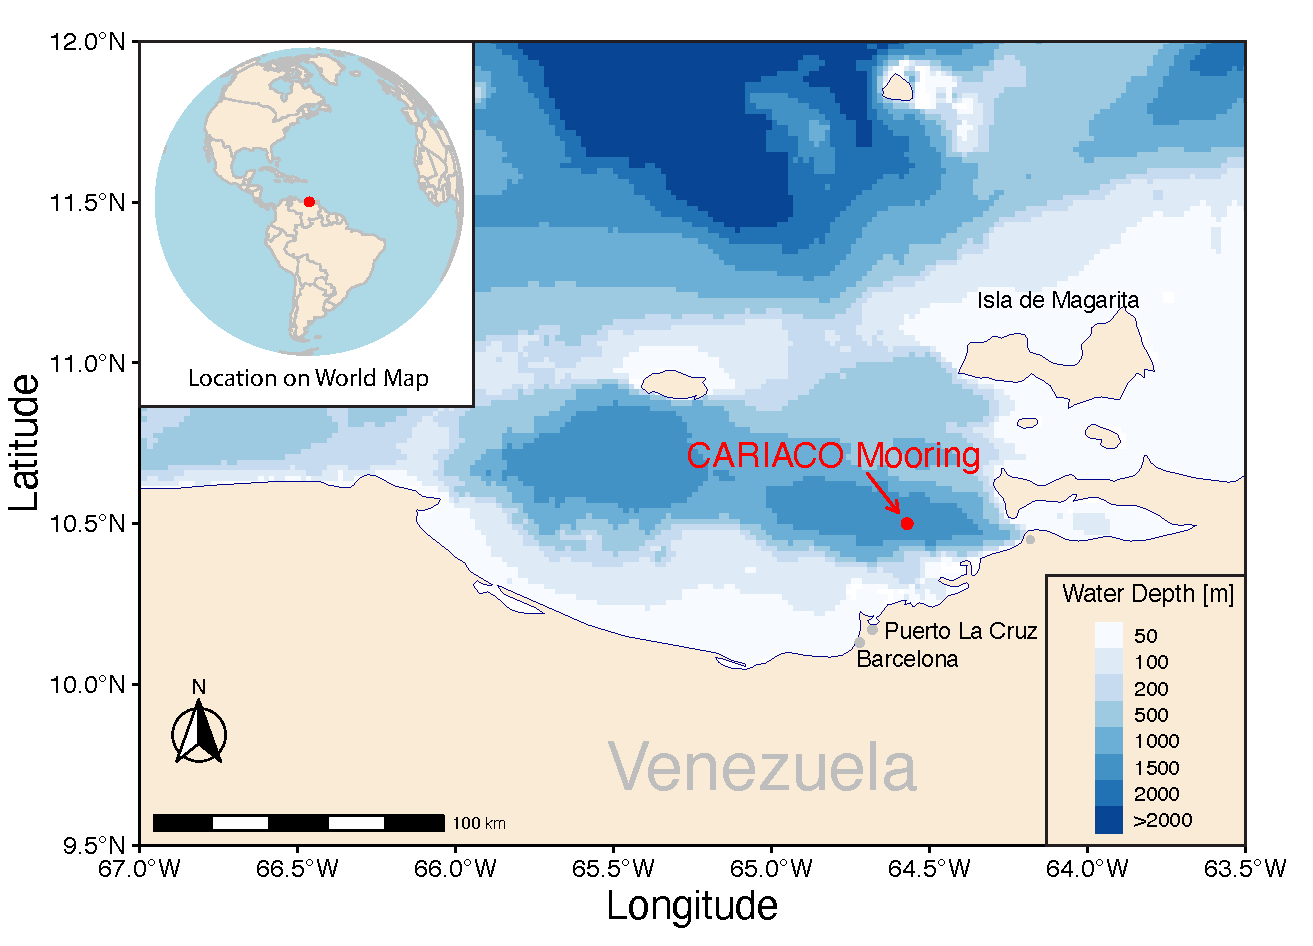
\includegraphics[width=\textwidth]{fig/Map_CAR.pdf}
\caption{Bathimetric map of the CARIACO Basin in the Caribbean Ocean, off the coast of Venezuela, indicating the CARIACO Mooring, the station of the Ocean Time-Series (located at \ang{10.50}N, \ang{64.67}W). A sill, running almost parallel to the coast at an average depth of \qty{100}{m}, from the Isla de Magarita and the Isla la Tortuga and beyond, encloses the Cariaco basin from the North.}
\label{fig:map}
\end{figure}


\subsection{In-Situ Data}
    Samples were collected as part of the Cariaco Ocean Time Series Program by means of monthly research cruises at a station located in the eastern Cariaco Basin (\ang{10.50}N, \ang{64.66}W) \cite{muller-karger_scientific_2019}.
    The CARIACO field program consisted of a monthly core oceanographic cruise with Niskin bottle and CTD deployments, along with other deployments and samples not utilized in this work. Field logistics and partial sample analysis were coordinated by the Fundación La Salle de Ciencias Naturales on Isla de Magarita, Venezuela. Details about the sampling procedures, analytical methods, data quality control, and inter-calibration procedures have already been described by \citeA{mullerkarger_annual_2001, thunell_particulate_2007, astor_yrene_m_handbook_2013, astor_interannual_2013, astor_sintesis_2014}. 
    
    All samples were collected using a 12-bottle rosette system equipped with a CTD (SeaBird, model SBE 25) \cite{astor_yrene_m_handbook_2013}. Water samples for chlorophyll a and nutrient analysis were taken monthly during the first cast of each cruise. These samples were collected at eight standard depths within the upper 100 meters (1, 7, 15, 25, 35, 55, 75, and 100 m). 

    Between late 1995 and early 1998, nutrient data was provided by William Senior (Universidad de Oriente, Cumana, Venezuela) and from mid-1997 to  present by Dr. K. Fanning (University of South Florida, St. Petersburg, USA). Samples from eight cruises were analyzed by both laboratories. Data for PO$_4$ and SiO$_4$ were in strong agreement (within ±5\%), whereas  NO$_\text{x}$ and NH$_4$ measurements showed discrepancies. \cite{taylor_ecosystem_2012}. We used a merged dataset for all nutrients, in which coincidental monthly measurements are averaged.
       
    For the identification of phytoplankton species by microscopy, \qty{500}{\milli\liter} seawater samples were collected at the same depths in HDPE bottles and preserved with a \qty{5}{\%} (final concentration) formalin solution neutralized with sodium tetraborate. Quantitative analysis was performed at the Universidad de Oriente, Venezuela, following the Utermöhl method \cite{hasle1978inverted}, using \qty{100}{\milli\liter} sedimentation chambers with a 48-hour settling period. Phytoplankton identification and enumeration by microscopy were restricted to microphytoplankton (cells $>$ \qty{20}{\micro \meter}) \cite{mutshinda_environmental_2013}.
    %from Mutshinda et al. 2013
    Quality control of the microscopy data was performed by assembling the taxonomic identifications made across all cruises, removing observations that were not identified at the species or genus level (with the exception of nanoflagellate cell counts) correcting spelling variations, and grouping synonyms using taxonomic information from the World Register of Marine Species (\url{marinespecies.org}). After processing the data, 482 phytoplankton species were observed over the course of the time series, which were grouped into 223 phytoplankton genera.

    
    Data collected with Niskin bottles, CTD, and phytoplankton taxonomy were retrieved from the Biological and Chemical Oceanography Data Management Office (BCO-DMO) \url{https://www.bco-dmo.org/project/2047}. 
    From the CARIACO Time Series data, we used only those variables that cover the entire length of the time series without large gaps (i.e. no more than three months) in coverage. In total, we used a complete set of 254 monthly data points, for which all variables were available.


\subsection{Climate data}
    %from Taylor et al. 2012
    Zonal wind stress (-u, easterly Trade Winds) across the southern Caribbean Sea drives nearshore upwelling of nutrient-rich waters via Ekman transport \cite{rueda-roa_southern_2013}. We extracted the -u wind component at \qty{10}{\meter} from the ECMWF Reanalysis v5 (ERA5) climate model and data reanalysis in the grid cell closest to the Cariaco time series sampling location (\ang{10.4}N, \ang{64.8}W, 31 km grid size), obtained from \url{https://cds.climate.copernicus.eu/datasets/reanalysis-era5-single-levels}. For simplicity, we refer to this variable as "wind speed" throughout the article. The data for precipitation and evaporation are also extracted from the ERA5 dataset for the aforementioned grid cell. Evaporation provides an estimate of the accumulated amount of water that has evaporated from Earth's surface, while precipitation is an estimate for total precipitation, comprising all water that falls on Earth's surface as rain or snow. 
    
    The monthly AMO index data (10-year low-pass), which represents area-averaged, detrended low-pass filtered North Atlantic SST anomalies, were obtained from \url{https://climatedataguide.ucar.edu/climate-data/atlantic-multi-decadal-oscillation-amo}. 
    
    The bi-monthly multivariate El Niño/Southern Oscillation (ENSO) indices (MEI v.2), defined as the time series of the leading combined Empirical Orthogonal Function (EOF) of five different variables (sea level pressure (SLP), sea surface temperature (SST), zonal and meridional components of surface wind, and outgoing long-wave radiation (OLR)) over the tropical Pacific basin (\ang{30}S-\ang{30}N and \ang{100}E-\ang{70}W), were obtained from \url{https://psl.noaa.gov/enso/mei/}. In our analysis, bi-monthly values are aligned with the tail month (December-January is treated as the value for January).
    

    \subsubsection{Data processing}
    % Niskin, CTD and Phytoplankton data processing
    Data were processed and analyzed using the R programming language (version 4.3.3) \cite{r_core_team_r_2024} with data pipelines created using tidyverse packages \cite{wickham_welcome_2019}. All the codes we produced for data processing and data analysis are publicly available on GitHub \url{https://github.com/ben1post/PhytoCariaco}.
    For all discrete depth measurements, the data were interpolated using the "oce" package \cite{kelley_oce_2023} with the adaptive "unesco" algorithm defined by the U.S. National Oceanographic Data Center \cite{johnson2006world}. The interpolated values were depth integrated to 100 meters and in four discrete intervals between 0-25, 25-50, 50-75 and 75-100 \meter for further analysis. Additionally, sea surface temperature (SST) was calculated from CTD temperature measurements averaged over the top \qty{10}{\meter}. For phytoplankton microscopy data, individually identified taxonomic units (species or genus) were interpolated and integrated across depth, and finally grouped by genus via the sum of interpolated counts.


\subsection{Data analysis}    
    To provide an overview of the available data and the general trends, we calculated annual means for relevant variables and normalized the data range as z-scores ($z = \frac{(x – \mu)}{\sigma}$). Cruises from 1995, 2016, and 2017 were excluded because insufficient coverage in these years prevented us from producing reliable yearly mean estimates. 
    
    As the main indicator of diversity, we used genus richness, thereby reducing taxonomic resolution to create a more homogeneous metric that is robust to discrepancies in sampling effort \cite{ptacnik_diversity_2008, de2020higher}. Furthermore, we calculated the Shannon index $H' = -\sum_i p_i \log_{e} p_i$ and Pielou's evenness $J' = -\sum_i p_i ln( p_i )/ln(H')$, where $p_i$ represents the genera observed for each interpolated and integrated monthly sampling. 

      
    \subsubsection{Analysis of Phytoplankton Community Structure}
    To investigate the structure of the phytoplankton community over time, we used a complete linkage clustering method via the "hclust" function in R \cite{r_core_team_r_2024} on the binary Jaccard distance matrix of annual aggregates of observed genera integrated over 100 m depth. Additionally, we performed non-metric multidimensional scaling (NMDS) ordination and hierarchical clustering on the monthly integrated counts that were square-root transformed using "metaMDS" from the "vegan" package \cite{oksanen_vegan_2024}. We employed the Bray distance matrix in a two-dimensional ordination that reached a converging solution within 30 steps. To relate the multidimensional structuring of the community data to variability in environmental data, we used the "envfit" function from the "vegan" package to fit the environmental vectors onto the ordination with 999 permutations. 
    To contrast the environmental parameters and diversity data between the community clusters resulting from the yearly aggregated clustering, we created density distribution plots contrasting the monthly measurements between clusters using the "ggpubr" package \cite{kassambara_ggpubr_2023}. To test whether the environmental variables, chlorophyll $a$ and diversity metrics varied significantly between the two community clusters, we employed a two-sided Wilcoxon sum rank test using the "wilcox.test" function in R \cite{r_core_team_r_2024}.
    % detailed explanation of NMDS in Winder and Hunter 2008

        
    \subsubsection{Assessing Environmental Drivers of Phytoplankton Dynamics}
    To quantify the effects of bottom-up drivers in the Cariaco Basin on shifts in the phytoplankton community, we employed a Gradient Forest analysis. Gradient Forest is a community-level extension of random forest analysis that combines regression trees calculated for indicator variables (here: monthly observed genus counts) to assess turnover in indicator variables across predictor variables \cite{pitcher_example_2012, large_critical_2015, tam_comparing_2017}. Gradient Forest calculates a goodness-of-fit statistic for each predictor variable and indicator variable, then it averages these to determine the overall importance of each predictor. The regression tree split values also identify the ranges of predictors in which significant changes occur in the indicator variables, signaling a threshold for phytoplankton community turnover. Cumulative plots of the predictive importance of each predictor variable can reveal thresholds for ecosystem drivers, as steep increases in cumulative importance signal a threshold for community turnover in the phytoplankton community \cite{tam_comparing_2017}. This analysis was conducted using monthly measurements integrated over a depth of 100 m for observed genus counts, ensuring the inclusion of all available data. The drivers/predictor variables considered in the analysis were the AMO index, the MEI v.2 index, wind speed, evaporation, precipitation, \qty{21}{\celsius} isotherm, SST, salinity, and nutrient concentrations ($\mathrm{[NO]}_3$, $\mathrm{[PO]}_4$ and $\mathrm{[SiO]}_4$). 
    The environmental variables from ocean time series tend to be strongly correlated, which the Gradient Forest methodology accounts for by implementing a conditional permutation of the correlated predictors \cite{ellis_gradient_2012}. 
    We show a model run without any time lags in  supplementary material (Figure \ref{fig:sup:GFoutput_nolags}). To consider the temporal lag in effect, particularly of climate indices, we included time lags of up to 6 months for all climate variables, as well as 3-month lags for in-situ measurements in exploratory runs. We chose time lags that scored highest in the goodness-of-fit statistics for the final model run (Table \ref{tab:sup:GFlagtests} in Appendix). 


    \begin{table}

\caption{Data and corresponding units used as predictor variables for the gradient forest analysis.}
\centering
\resizebox{\textwidth}{!}{\begin{tabular}[t]{rrl}
\toprule
Variable Name & Units  & Data source \\
\midrule
MEI v.2 & unitless & Climate index provided by NOAA \\
AMO & unitless & Climate index provided by NSF NCAR \\
Wind speed & \qty{}{\meter/\second} & ERA5 model reanalysis, negative 10 m u-component of wind speed \\
Precipitation & \qty{}{\meter} & ERA5 model reanalysis, total precipitation\\
Evaporation & \qty{}{\meter} & ERA5 model reanalysis, evaporation \\
SST & \qty{}{\celsius} & CTD, Average temperature measured down to \qty{10}{\meter} depth\\
\qty{21}{\celsius} isotherm & \qty{}{\meter} & CTD, depth at which temperature reaches 21°C\\
Salinity & PSU & Niskin, interpolated down to \qty{100}{\meter} depth \\
$\mathrm{NO}_3$  & µM & Niskin, interpolated down to \qty{100}{\meter} depth \\
$\mathrm{PO}_4$  & µM & Niskin, interpolated down to \qty{100}{\meter} depth \\
$\mathrm{SiO}_4$  & µM & Niskin, interpolated down to \qty{100}{\meter} depth \\
\end{tabular}}
\label{tab:DataSources}
\end{table}


\section{Results}

% Figure 2
Figure \ref{fig:zscore} shows the normalized yearly means of all environmental variables considered, the logarithmic transformation of chlorophyll \textit{a}, and phytoplankton cell counts per functional group. We included marks to highlight years with a significant number of missing monthly measurements ($=$ 2, 3 months and $\geq$ 4 months), since these make the annual means less reliable. Particularly toward the later years of the time series, the sampling became sparse. The patterns emerging from wind speed, evaporation, precipitation, SST, and \qty{21}{\celsius} isotherm depth clearly show the years of positive anomalies of wind (blue) and negative anomalies for SST (red) and upwelling (red, i.e., shallower depth of the isotherm). These patterns are reflected in the mode of the AMO, where a positive anomaly correlates with weak upwelling regimes (see also Figure \ref{fig:sup:correlation} in Appendix). The yearly mean nutrient concentrations have a maximum positive anomaly at the start of the time series but show differing inter-annual oscillations. Annual mean anomalies of nitrate and phosphate appear to follow upwelling anomalies but remain relatively low between 2002 and 2014, with some variability in mean phosphate concentration. Silicate does not follow a clear pattern but shows an elevated mean concentration between 2008 and 2013, which could be driven by increased surface runoff \cite{lorenzoni_characterization_2015} and reduced depletion due to diminished diatom abundances.

\begin{figure}
\noindent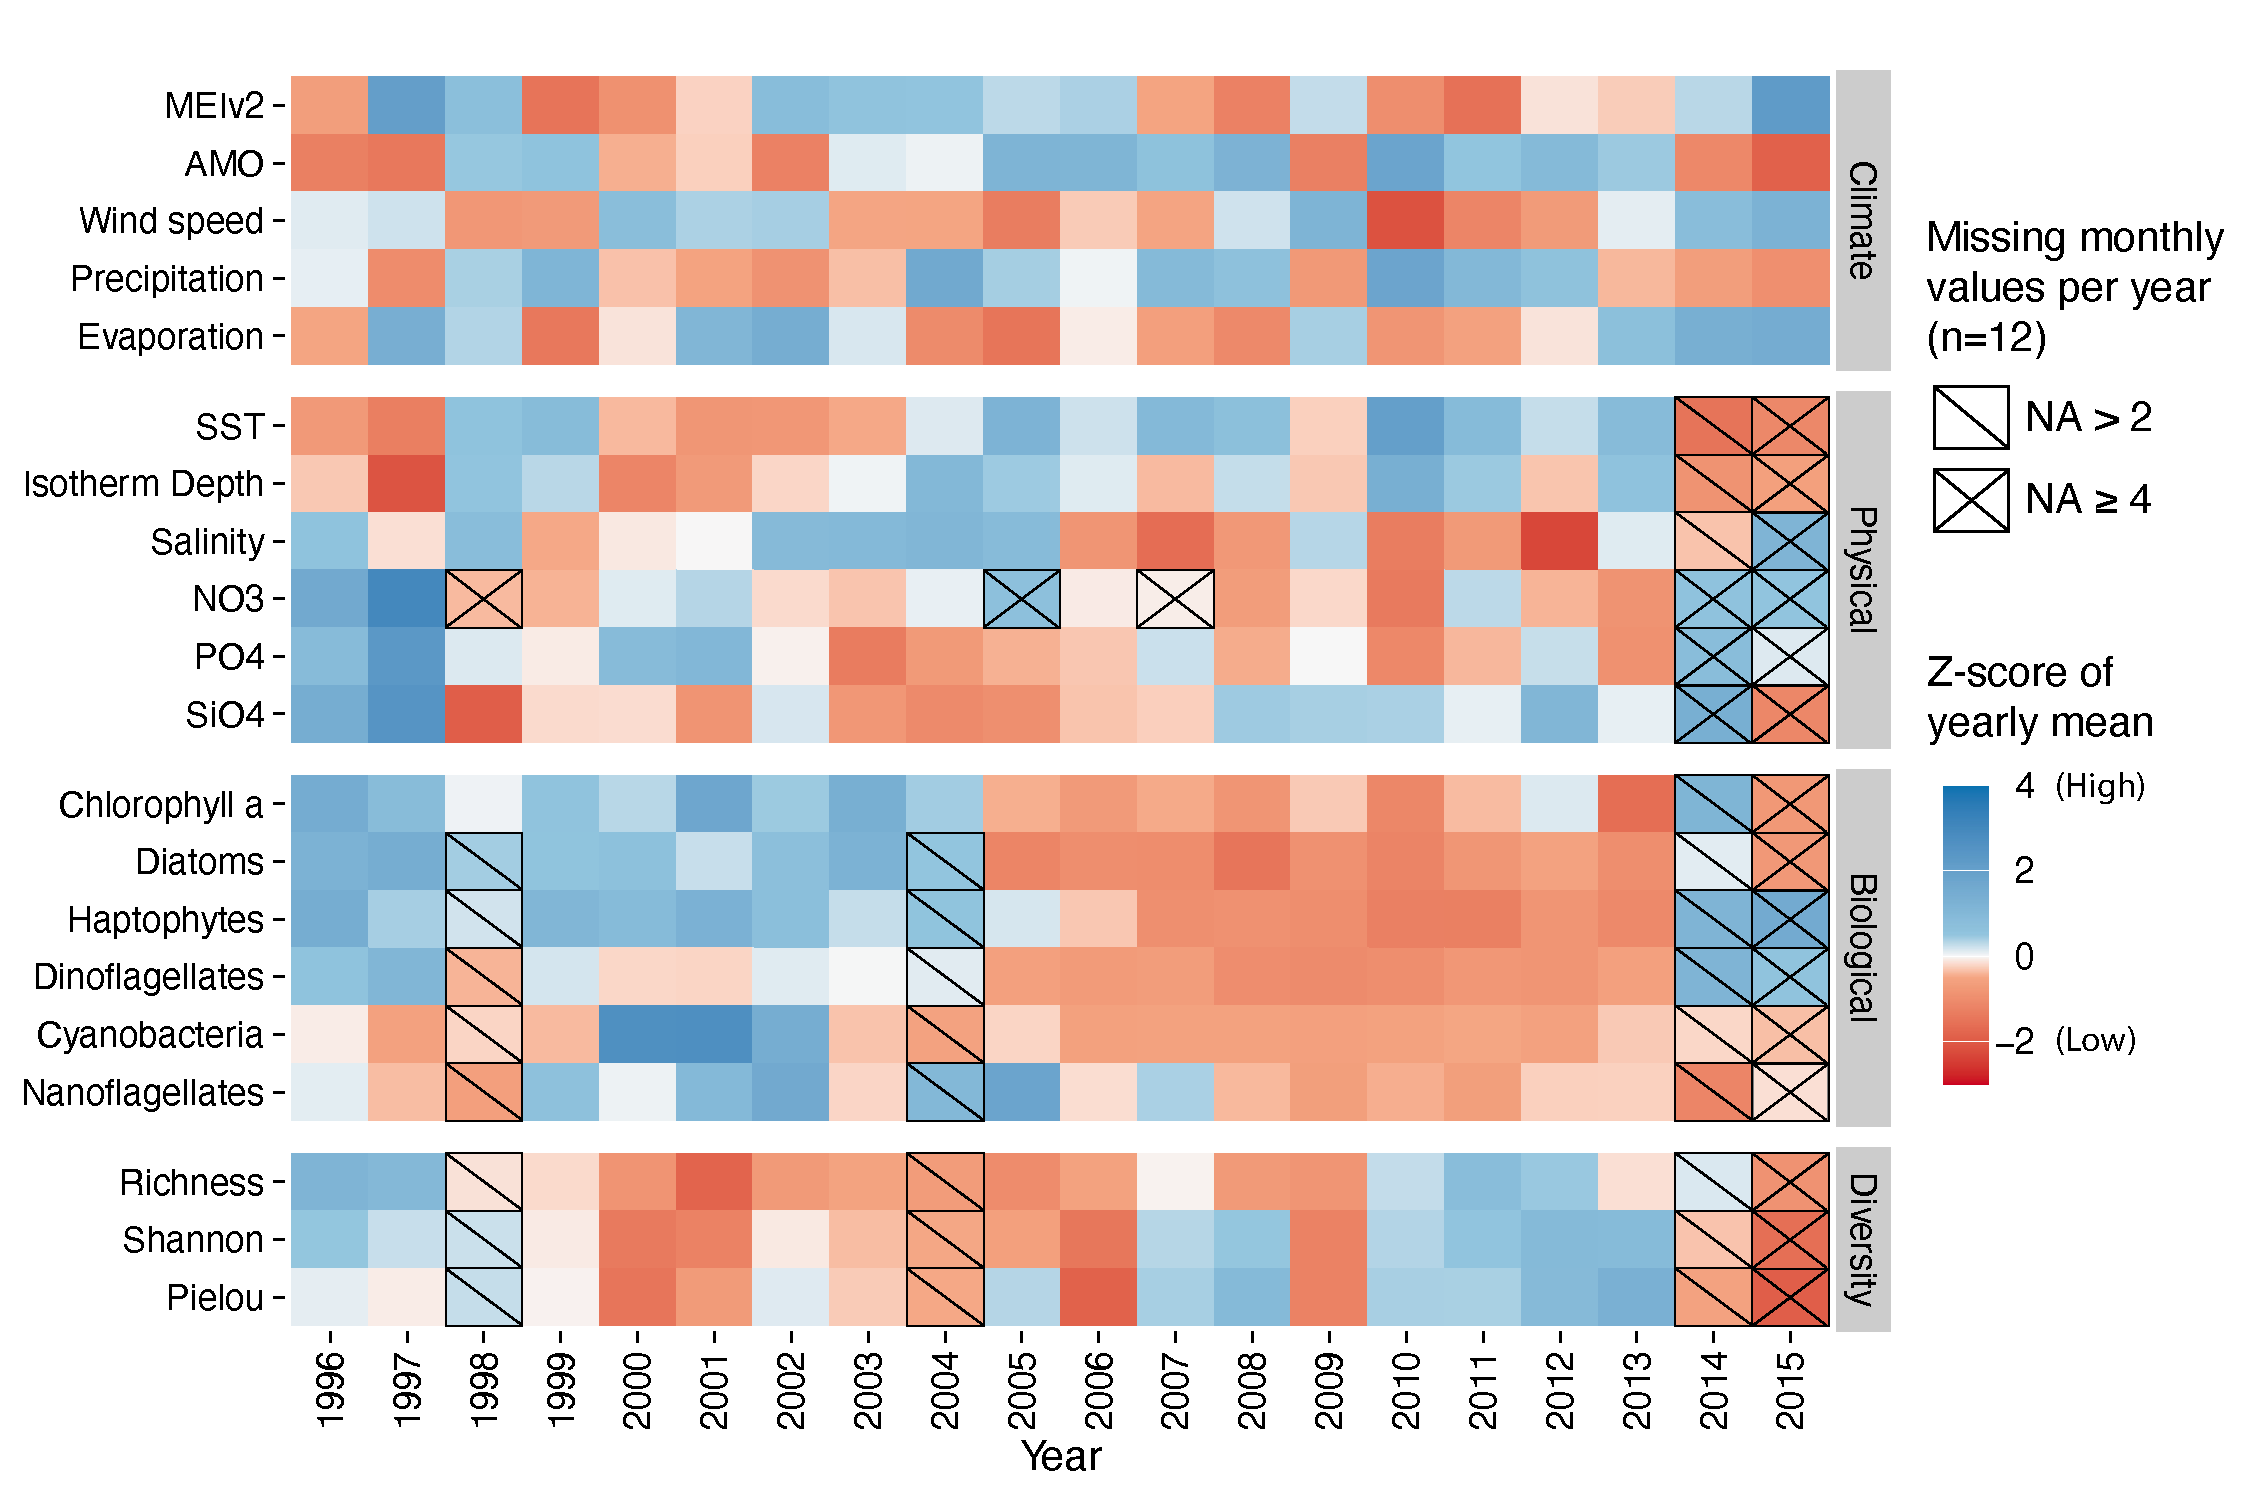
\includegraphics[width=\textwidth]{fig/Figure2_ZScores_v2.pdf}
\caption{Time series showing annual z-scores of selected indicator and driver variables. Red indicates negative annual anomalies and blue indicates positive annual anomalies. Deeper shades indicate larger anomalies. All data are available at monthly resolution. The years 1995 (n=2) and 2016 (n=5), 2017 (n=1) were removed due to lack of data, additionally we marked years with two or three and four or more missing values to highlight unreliable annual mean estimates. Diversity Indices are calculated based on microscopy counts at the Genus level.}
\label{fig:zscore}
\end{figure}

% Figure 3
Figure \ref{fig:divts} shows the depth distribution and dynamics of chlorophyll \textit{a} and community diversity indices, also in relation to rainy and upwelling seasons. The bulk of the chlorophyll \textit{a} biomass ($\sim$ 80\,\%) was measured in the upper 50 meters of the water column, with approximately 15\,\% measured between 50 and 75 meters. Chlorophyll \textit{a} exhibits marked seasonality, with the highest biomass in the upper water column during the winter months (December–February, Figure \ref{fig:divts}$b$). The yearly mean chlorophyll \textit{a} biomass shows the highest variability within the upper 25 meters. In some years, particularly in 2000, 2005, 2007, 2008, and 2013, the concentration in this layer was lower than in the 25–50 meter depth range (Figure \ref{fig:divts}$a$). In general, yearly mean anomalies within the upper 75 meters appear to be high during the period from 1996 to 2004 and only reduces in 2012. The year 2013 is an outlier, particularly for the upper 25 meters, as the missing monthly samplings from the winter months (January and February) skew the value. Nevertheless, the monthly measurements for the remainder of the year 2013 show a markedly lower biomass (65\,\% of the mean over the entire time series for these months), which recovers in 2014. Chlorophyll \textit{a} biomass below 50 meters depth shows a relatively stable distribution throughout the year and across the time series. In fall, during the rainy season, mean chlorophyll \textit{a} biomass in the upper 25 meters is markedly reduced, while the 50–75 meter depth interval shows a slight increase, indicating a shift in the chlorophyll \textit{a} maximum to lower depths under weak upwelling conditions.
The calculated genus diversity from the microscopy cell counts generally follows the dynamics of chlorophyll \textit{a} biomass, with maximum values observed during the upwelling seasons in winter. Genus richness is consistently the highest diversity index in the top \qty{25}{meters} depth interval, and shows also the highest variability over the time series. Across the time series, we observe maximum richness at the start of the time series (1996-1997), with a subsequent reduction in diversity across all depths, with a recovery after 2011. The  reduction in diversity following the start of the time series does not follow the pattern shown by chlorophyll \textit{a}, which remains relatively stable across the top \qty{100}{meters} until 2004 (see Figure \ref{fig:divts $a$}). Scaling this genus diversity by the cell count abundances, i.e. the Shannon index, shows a similar but less pronounced dynamic. Diversity remains high throughout 2000 and recovers more quickly but shows marked reductions in annual means, particularly in the upper 25 meters in 2006, 2009, and 2016. The seasonal signal is lost (see Figure \ref{fig:divts} $f$). 
Community evenness, expressed by the Pielou index, shows no seasonal signal and a very large variance within seasons and through depth (see Figure \ref{fig:divts} $h$). The inter-annual dynamics of evenness are remarkably stable across all depth intervals, clustered around an intermediate 0.5 value. There are marked reductions in all depths towards 2000 and for all depths above 75 meters in 2006, 2009 and 2016. Throughout 2003 to 2013 evenness is almost consistently highest in the deepest interval below 75 meters, where the community seems to have been more evenly distributed. 


\begin{figure}
\begin{center}
\noindent\includegraphics[width=480pt]{fig/DepthDivTimeSeries_updated.pdf}
\end{center}
\caption{Time series and seasonality of chlorophyll \textit{a} and diversity indices at four depth intervals. (a,c,e,g) Large dots and lines mark annual mean across time series for years with more than 5 monthly sampling. Small, transparent dots show monthly raw values. (b,d,f,h) Boxplots of monthly measurements at four depth intervals grouped by season. Upwelling season goes from December to May, Rainy Season from June to November.}
\label{fig:divts}
\end{figure}


% Figure 4
We undertook clustering analysis on annually aggregated cell counts from microscopy and on individual monthly measurements. Figure \ref{fig:clustering}$a$ shows the results of clustering the annually aggregated communities using a linear complete linkage algorithm based on the binary Jaccard matrix. Two distinct clusters emerge from this analysis, with the first cluster encompassing the years 1996-2004 and 2014-2016, and the second cluster including the intermediate years from 2005 to 2013. 
Inter-annual species turnover is shown in Figure \ref{fig:clustering}$b$, it reveals an increasing trend in turnover from 1996 to 2004. Turnover subsequently decreases during the period underpinning cluster 2 and increases again in 2014, marking a return to cluster 1. This pattern is also reflected in the hierarchical clustering results, Figure \ref{fig:clustering}$a$, where cluster 2 shows a lower distance in the clustering tree between the years. We additionally extracted the three dominant genera for the second cluster and the early and late parts of the first cluster, respectively. The diatom \textit{Thalassiosira} dominated the early period and was abundant in all other periods. \textit{Pseudo-nitzschia} dominates cluster 2, with the haptophyte \textit{Emiliana} being the second most abundant genus. The later part of cluster 1 is dominated by \textit{Emiliana}. 

To check whether the annual aggregation of community data smoothed out strong seasonal signals, we performed an NMDS cluster analysis using the monthly cell counts (Figure \ref{fig:clustering}$c$). The NMDS clustering is overlaid with environmental data and climate indices in an attempt to unveil some of the underlying trends. The horizontal axis separates the two clusters, with cluster 2 located over positive anomalies in AMO and precipitation, and cluster 1 located over positive anomalies in evaporation, salinity, and MEI v.2. The second NMDS axis appears to follow the trends in upwelling intensity, as indicated by the vectors pointing in opposite directions for nutrient concentrations, temperature, and wind speed. Overall, the NMDS clustering confirms the pattern shown by clustering on annually aggregated data. 

\begin{figure}
\noindent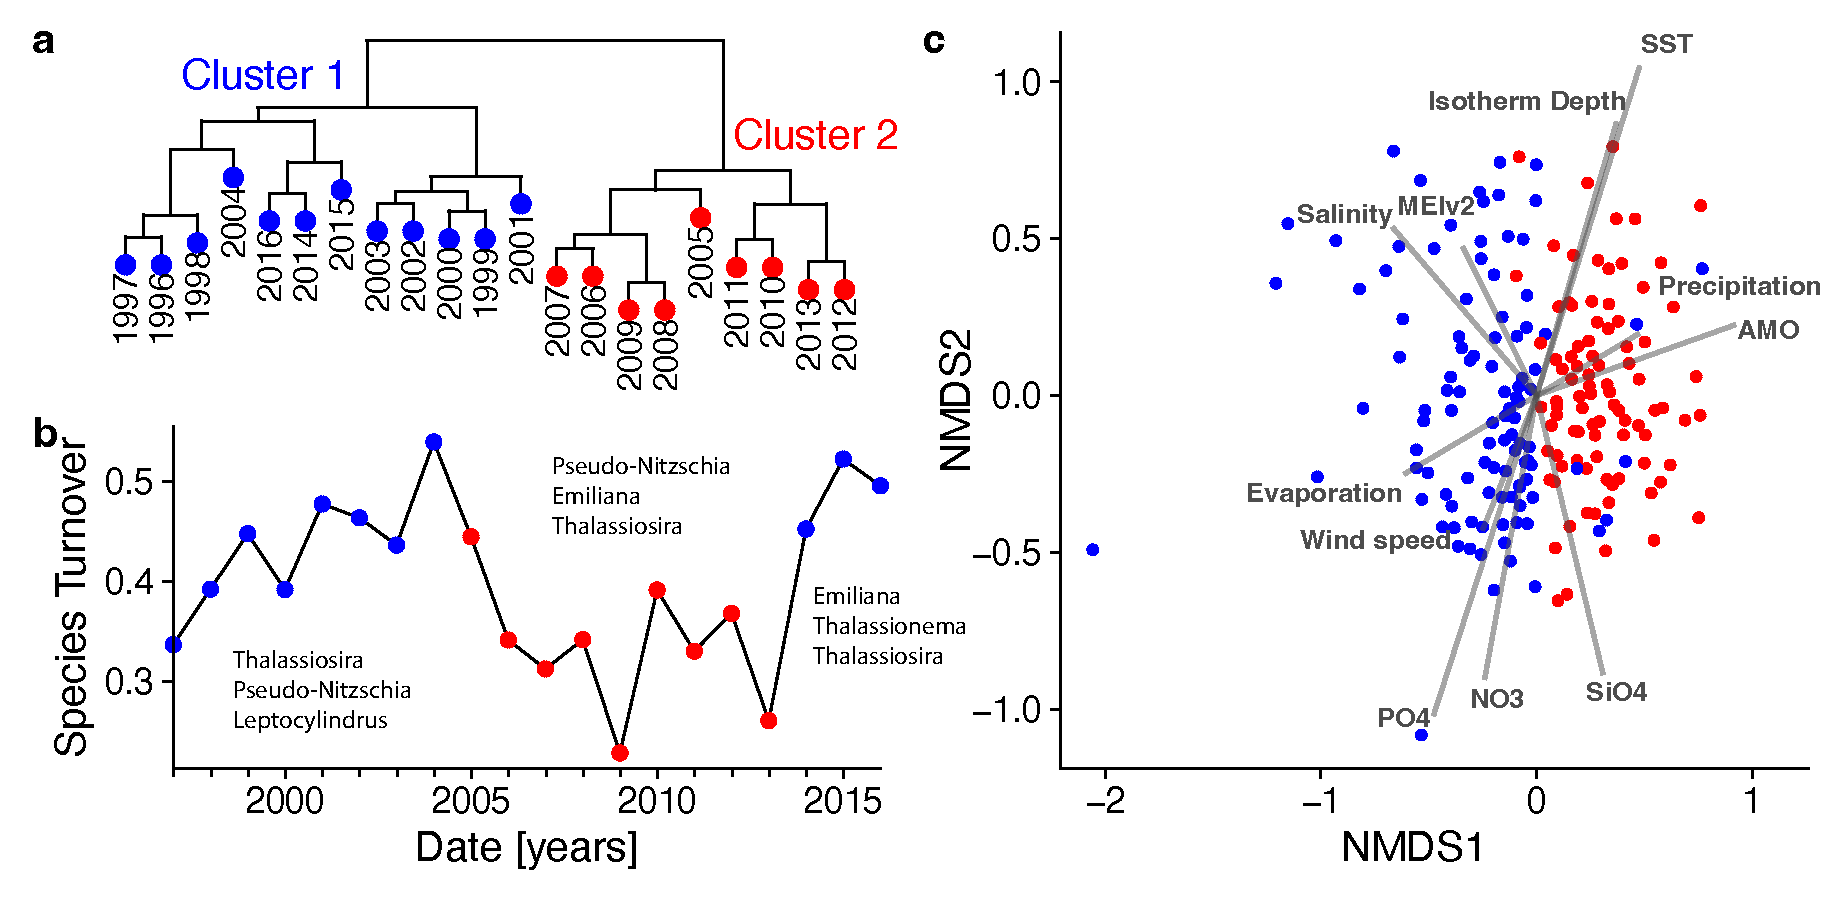
\includegraphics[width=\textwidth]{fig/Figure4_ClusteringNMDS_v2.pdf}
\caption{(a) Hierarchical clustering by complete linkage method of microscopy cell counts at the Genus level, using the binary Jaccard distance. The community for each year is binned together, to smooth out seasonal features. (b) Species turnover between years for annual aggregate of identified phytoplankton to a genus level. The three genera dominating the cell counts for the separate parts of cluster 1 and cluster 2 are given in order of abundance from top to bottom. (c) NMDS plot of monthly community data (cell counts) that is cube-root transformed. Stress: 0.261, 2 dimensions, converging solution. The dots are color-coded based on the cluster they belong to. Vector overlay of ENVFIT shows how environmental variables are co-varying with community data. Length of vector indicates strength of relationship.}
\label{fig:clustering}
\end{figure}

% Figure 5 - NEW
Figure \ref{fig:clustcomp} shows density distributions of environmental variables, chlorophyll \textit{a}, and diversity indices for the two clusters. Upwelling-related variables exhibit distinct patterns between the two clusters. For example, cluster 1 experiences more frequent high wind events, a shallower \qty{21}{\celsius} isotherm, lower temperatures, reduced evaporation, and higher salinity and nutrient concentrations, particularly for nitrate. The AMO index shows a pronounced separation between the two clusters, with cluster 1 exhibiting more negative anomalies, while cluster 2 shows a higher occurrence of positive anomalies. Although there are no significant differences in genus richness and the Shannon index between clusters, there is a slightly increased median in the Pielou index for cluster 2 (Table \ref{tab:ClustCompWilcox}). The density distribution reveals some differences. Cluster 1 shows higher variance for genus richness, while cluster 2 shows greater variance and a bimodal distribution for the Shannon and Pielou indices. 

\begin{figure}
\noindent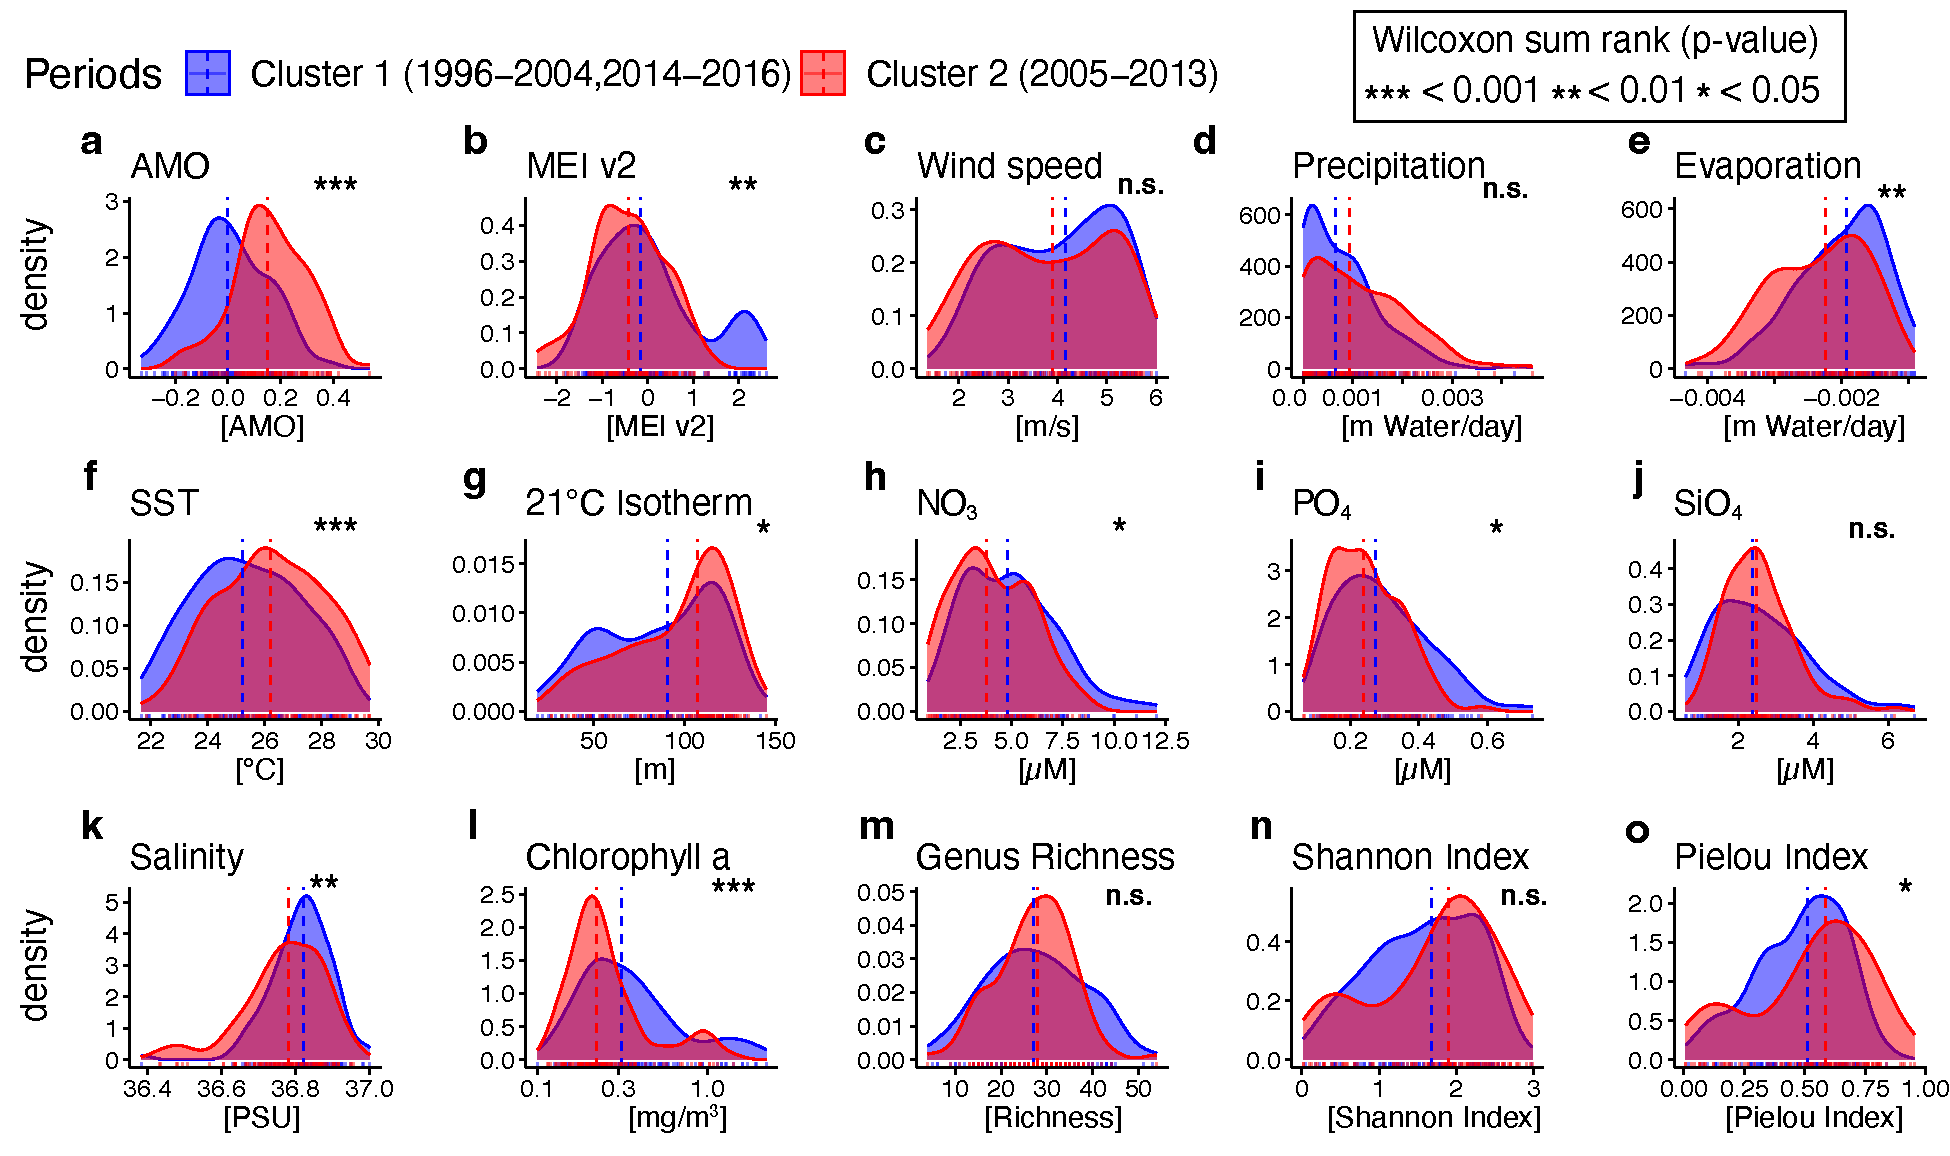
\includegraphics[width=\textwidth]{fig/Figure5_ClustCompPlot_v2.pdf}
\caption{Density distributions of environmental variables, chlorophyll \textit{a}, and diversity indices for the two clusters. The dashed lines mark the median of each distribution. Significance levels of Wilcoxon sum rank tests between clusters are shown above plots  (p-value: ***\textless0.001, **\textless0.01, *\textless0.05, n.s.=not significant).}
\label{fig:clustcomp}
\end{figure}


% Figure 6
To identify the variables that best predict the shifts observed within the phytoplankton community, we performed a Gradient Forest analysis on the microscopy cell counts interpolated over the top 100 meters and grouped by identified genus. Preliminary model runs were used to determine whether time lags of the predictor variables could better explain the data (see Appendix), resulting in the selection of the AMO with a lag of 2 months and MEI v.2 with a lag of 4 months. Figure \ref{fig:GF}$a$ shows the predictor variables ranked by their weighted importance, with the AMO and MEI v.2 indices with time lags, as well as upwelling-related variables such as SST and nitrate in the upper 100 meters, demonstrating the highest predictive capacity. The \qty{21}{\celsius} isotherm, precipitation, and phosphate concentrations scored the lowest in predicting changes within the community. Gradient Forest predicts shifts in the community by building a random forest model for each observed genus across the time series. The predictive power of the models for each genus is shown in Figure \ref{fig:GF}$b$. The microscopy data are biased toward larger cell sizes and, therefore, most of the predicted genus cell counts are from diatoms. However, two haptophyte and three dinoflagellate genera rank relatively high.
Figure \ref{fig:GF}$c$ shows the cumulative importance of the predictor variables across the parameter range. The black, dashed lines indicate cumulative importance across the entire community, and the solid, dashed lines indicate importance per phytoplankton group. For the AMO index, we see a clear pattern in which negative anomalies affect the community. This contrasts with a higher importance for positive anomalies in the MEI v.2 index, particularly for haptophytes and cyanobacteria. Nitrate concentrations between 6 and 8 \unit{\micro \mole} represent the range within which the community changed most, indicating these values as a threshold for community composition. Figure \ref{fig:sup:GFoutput_lags_extra} in Appendix shows response curves for all variables not shown here. For wind speed, SST, and salinity, changes occurred mostly within parameter ranges related to high upwelling, i.e., high wind (between -4 and -6 \unit{m.s^{-1}}), low temperature (below \qty{23}{\celsius}), and high salinity (above \qty{36.8}{PSU}). 

\begin{figure}
\noindent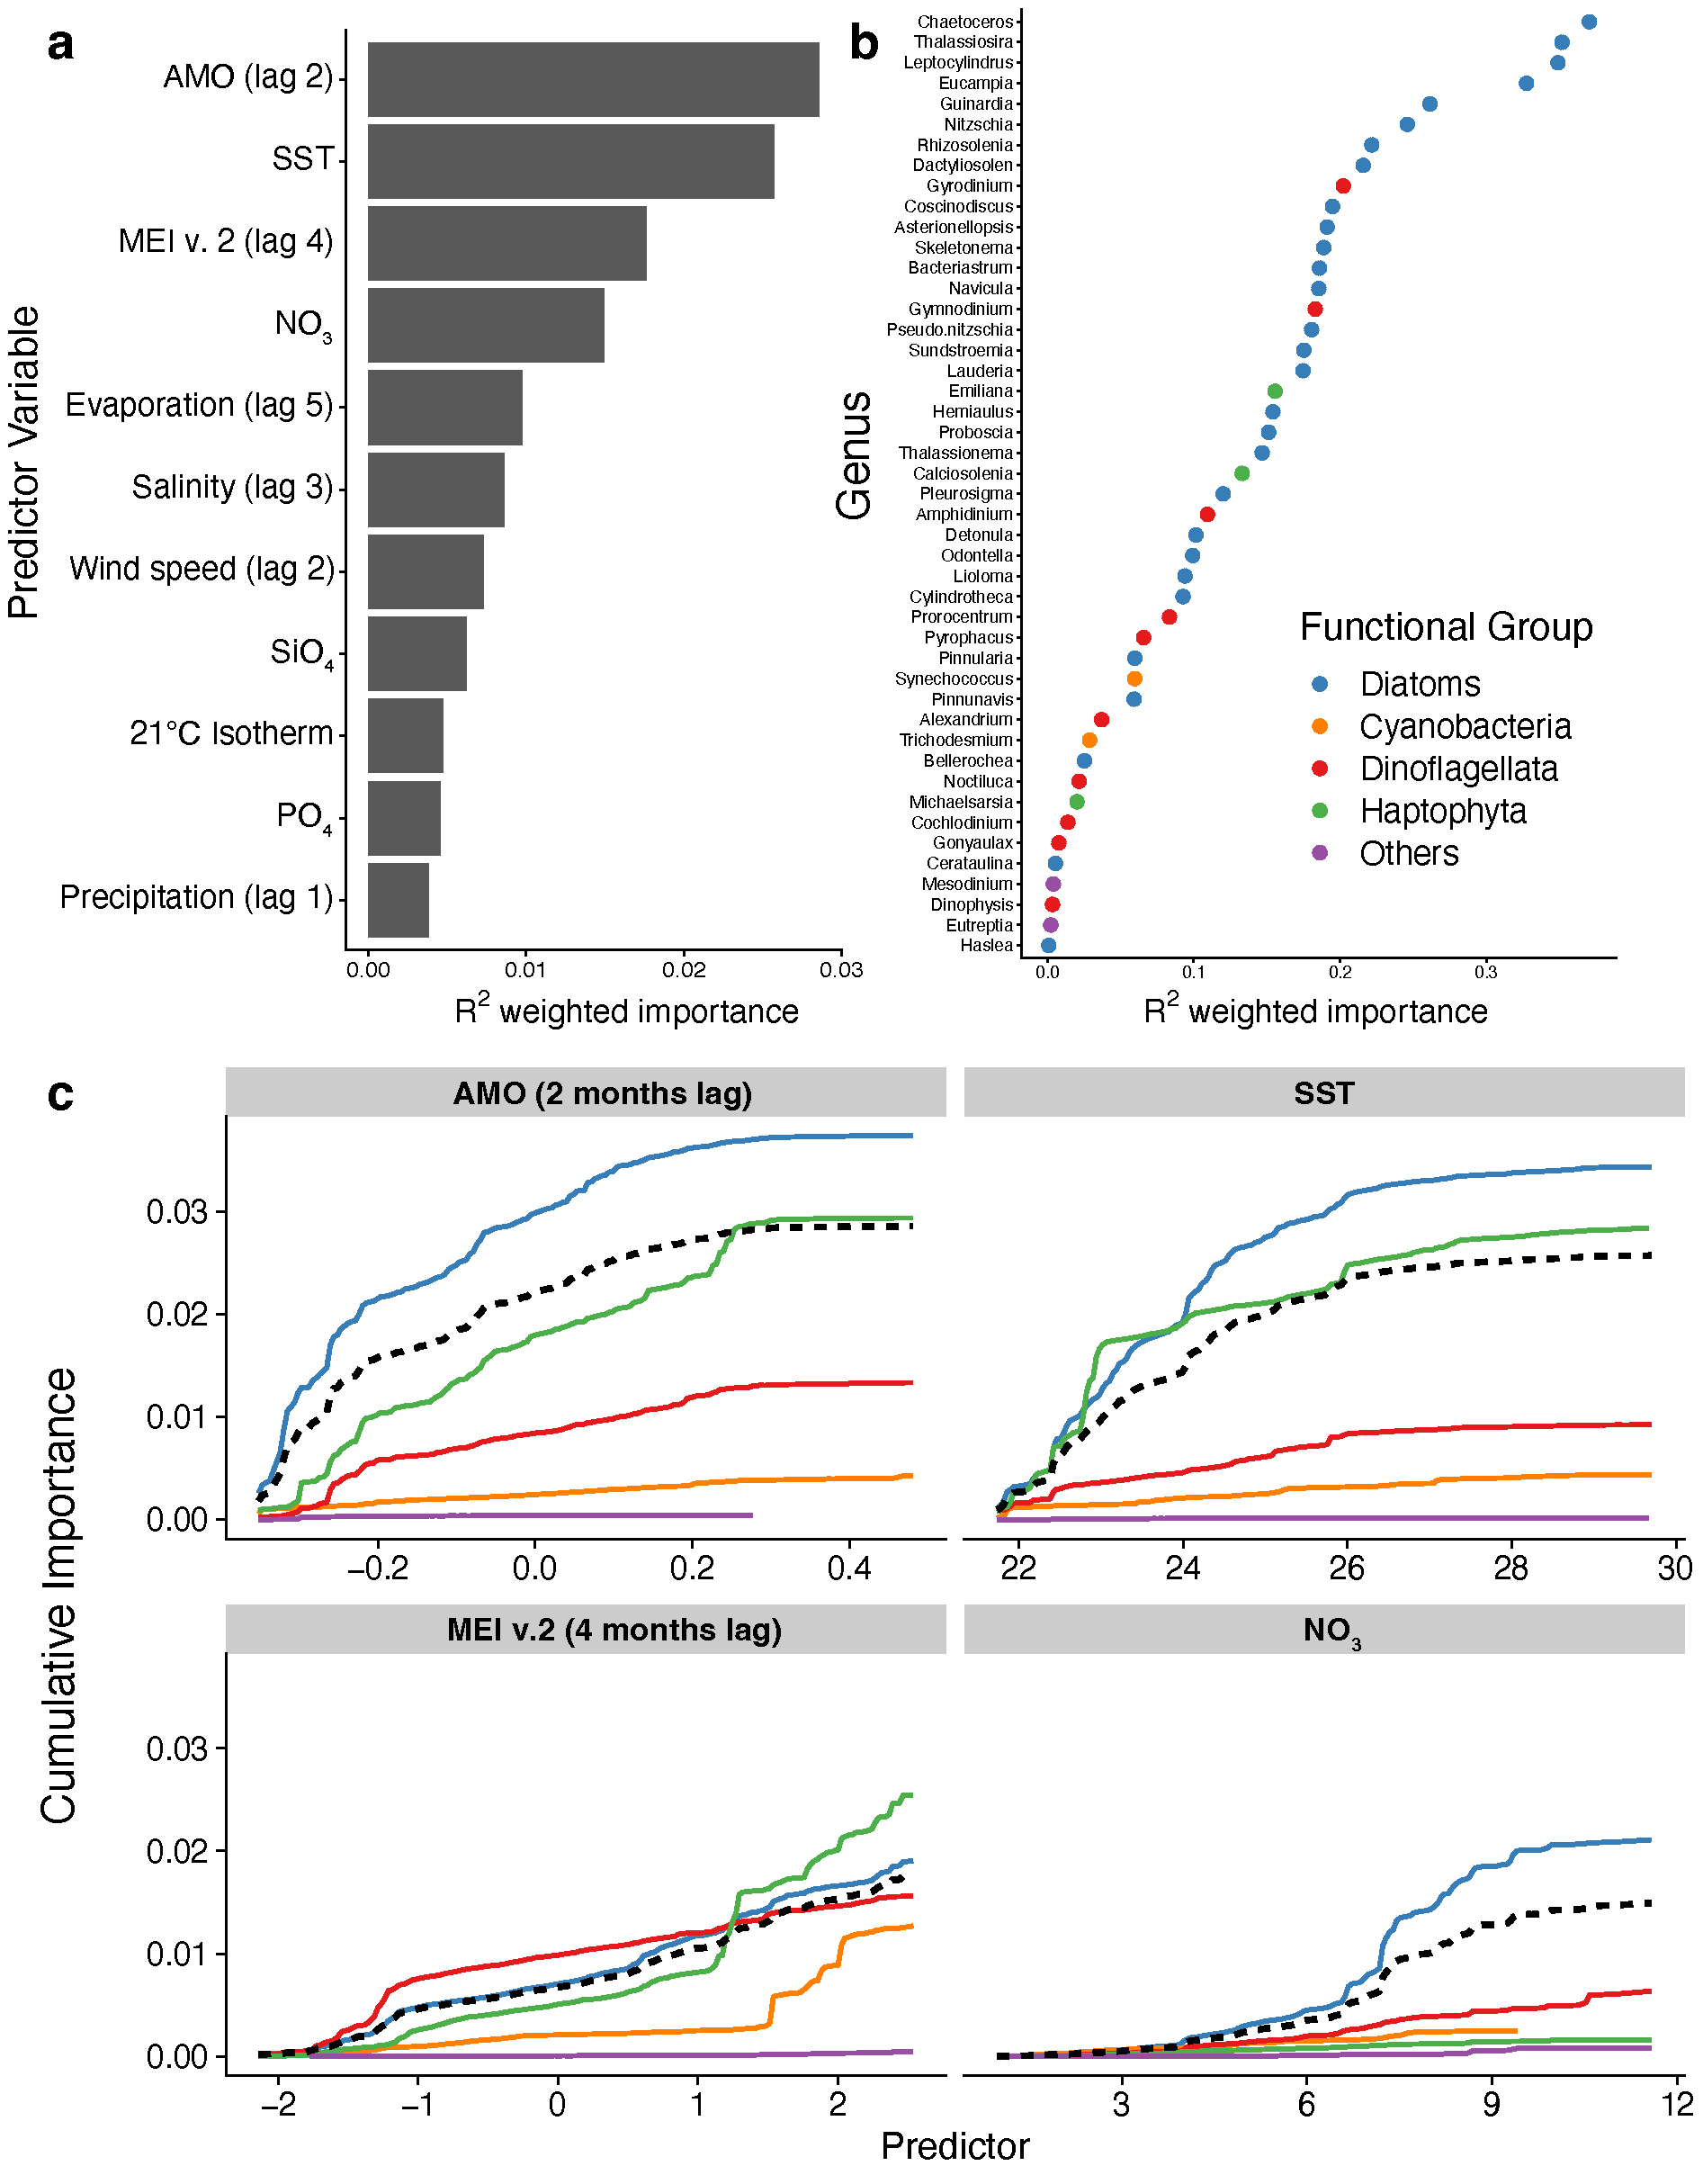
\includegraphics[width=\textwidth]{fig/Figure6_GF_output_FINAL_v2.pdf}
\caption{Gradient Forest analysis of monthly community data at a genus level. (a) Predictor variables ranked according to overall weighted importance in predicting shifts in abundances. (b) Phytoplankton genera that could be predicted ranked according to the predictive power via the weighted importance. (c) Cumulative importance curves for the predictor variables. Black line shows cumulative importance across predictor range for the entire model and all genera. Dashed colored lines represent the responses of individual functional groups.}
\label{fig:GF}
\end{figure}


\begin{table}
\caption{Results of two-sided Wilcoxon sum rank test with continuity correction for variables between the two clusters. Cluster 1 covers the periods 1996-2004 and 2014-2016 and cluster 2 covers the period 2005-2013.}
\centering
\begin{tabular}[t]{lrrl}
\toprule
Variable & W & p.value & Significance\\
\midrule
AMO & 3494.0 & 1.86e-14 & ***\\
MEI v.2 & 9523.5 & 0.006 & **\\
Wind speed & 7074.0 & 0.143 & n.s.\\
Precipitation & 6251.0 & 0.004 & **\\
Evaporation & 9979.0 & 3.68e-5 & ***\\
\addlinespace
21 °C Isotherm & 5293.0 & 0.034 & *\\
SST & 4712.0 & 0.001 & ***\\
Salinity & 7636.0 & 0.002 & **\\
$NO_3$ & 6378.0 & 0.018 & *\\
$PO_4$ & 7359.0 & 0.012 & *\\
$SiO_4$ & 5998.0 & 0.736 & n.s.\\
\addlinespace
Chlorophyll $a$ & 8229.0 & 9.63e-6 & ***\\
Genus Richness & 5913.0 & 0.954 & n.s.\\
Shannon Index & 5142.0 & 0.108 & n.s.\\
Pielou Index & 4874.0 & 0.029 & *\\
\bottomrule
\end{tabular}

\label{tab:ClustCompWilcox}
\end{table}



\section{Discussion}

\subsection{Community reorganization and biomass shifts}
% P1: Introductory paragraph highlighting the overall dynamics/shifts
This study demonstrates the highly dynamic nature of a tropical coastal marine ecosystem driven by local environmental variability, which is, in turn, influenced by large-scale climatic changes. In the Cariaco Basin, decadal-scale climate oscillations impacted the wind-driven upwelling regime, producing confounding effects on the composition and biodiversity of the phytoplankton community.
These changes are well visible in the yearly mean anomalies (Figure \ref{fig:zscore}) and the density distribution of monthly measurements (Figure \ref{fig:clustering}). After 2004, we observed increased sea surface temperatures (SST), decreased wind speeds, reduced fluorometric chlorophyll \textit{a}, and drastically reduced cell counts of functional groups, all coincident with a shift in the Atlantic Multidecadal Oscillation (AMO) toward positive mean anomalies up to 2014. 
By considering the phytoplankton community time series until the end of 2017, the temporally complete dataset, we find that the observed shift that occurred in 2004 produced a temporary regime that lasted only until 2014 (cluster 2), when the system reverted to the precedent regime of 1996-2004 (cluster 1), confirming the observations by \citeA{muller-karger_scientific_2019}. In 2014, physical conditions in the Cariaco Basin returned to a regime of increased wind speed, increased upwelling, and elevated nutrient concentrations (Figure \ref{fig:zscore}). Concurrently, we observe an increase in chlorophyll \textit{a} (Figure \ref{fig:divts} $a$) and a return to a community composition more similar to the period between 1996 and 2004 (Figure \ref{fig:clustering} $a$ and $c$).

% P2: Discuss community reorganisation, biomass shifts vs HPLC data 
When comparing the two regimes, we observe a marked reduction in cell counts, which corresponds to a decreased concentration of chlorophyll \textit{a}, particularly in the top \qty{25}{meters} of the water column (see Figure \ref{fig:divts}). The decline in cell counts was not proportional to the more modest decrease in total chlorophyll \textit{a}, suggesting that the phytoplankton community might have transitioned to smaller cells, which were probably below the detection size limit of optical microscopes \cite{muller-karger_scientific_2019}. This shift to smaller cell sizes and a reduction in diatoms is consistent with predicted effects of warming and reduced mixing on phytoplankton communities \cite{bopp_response_2005}. Increases in temperature can lead to a decrease in the relative contribution of large cells in the community, irrespective of nutrient availability, but shifts towards smaller cells are particularly prevalent when temperatures increase and nutrient supply decreases \cite{mousing_global_2014}, as we observed in the Cariaco Basin. 

% Disucssion of HPLC vs Microscopy!
A similar pattern emerges when comparing our observations with High-Performance Liquid Chromatography (HPLC) data from the Cariaco Basin, which were analyzed and presented by \citeA{pinckney_phytoplankton_2015}. The HPLC data suggest an increase in chlorophyll \textit{a} between the periods 1996-2000 and 2006-2010, particularly at depths below \qty{55}{meters} \cite{pinckney_phytoplankton_2015}. Despite cell counts of all functional groups decreasing, the HPLC data indicate an increase in non-diatoms and a redistribution of biomass to depths below \qty{55}{\meter}. This is a further strong indication that the phytoplankton community shifted to smaller sizes, undetected using light microscopy.
It should be noted that the HPLC data were analyzed by multiple laboratories throughout the time series, with a gap in data coverage between 2000 and 2006. \citeA{pinckney_phytoplankton_2015} could not find a consistent method for quantifying total chlorophyll \textit{a} across different laboratories. This is why we focused our analysis on the more consistent and temporally complete microscopy cell count and fluorometric chlorophyll \textit{a} data.
Consistent with our results, independent spectrophotometric measurements of chlorophyll \textit{a} concentrations at \qty{20}{meters} depth, off the coast of Margarita Island, show a reduction in chlorophyll concentration between 2004 and 2014 \cite{gomez_gaspar_variacion_2025}.


% P3: Shift in Diversity does not match shift in biomass/cell counts, why?
The temporal dynamics we find in yearly mean genus richness, however, do not correspond directly to the observed regimes. Instead, we see a marked reduction from 1998 to 2010, after which richness recovers four years prior to 2014, when the community returns to levels characteristic of regime 1. The same trend is evident, albeit to a lesser degree, in the other diversity metrics. Generally, mean annual anomalies in Shannon diversity and Pielou's evenness correlate with genus richness and exhibit a reduced yearly mean between 2000 and 2006, during which cell counts recorded an increase in nanoflagellates and a pronounced peak in cyanobacteria.
We did not find a significant difference in diversity between the two regimes, either by Shannon index or by genus richness (Figures \ref{fig:zscore} and \ref{fig:divts}). However, we did observe a significant difference in Pielou's index between the two regimes. The results suggest that the phytoplankton community becomes more evenly distributed during low-upwelling conditions of regime 2, which is consistent with the analysis of \citeauthor{pinckney_phytoplankton_2015} based on HPLC pigment data. This increase in evenness, quantified by the Pielou index, is most likely explained by the lack of strong upwelling events and the resulting reduced disturbance of the community. The resulting decrease in compositional turnover is also observed in a decline in interannual species turnover during regime 2 (see Figure \ref{fig:clustering}$b$). As the productivity and biomass of phytoplankton communities are driven primarily by nutrients supplied through disturbance events, this confirms the previously observed inverse relationship between evenness and community performance \cite{lehtinen_phytoplankton_2017, otero_phytoplankton_2020}.



\subsection{Drivers of change}
% P4: Introduce GF Analysis and discuss results
To identify the variables that best predict changes in the phytoplankton community, we conducted a gradient forest analysis using time series of climate indices and in situ measurements to predict genus-level abundances from microscopy cell counts. Gradient forest is an extension of the random forest algorithm, designed to identify thresholds and patterns in community composition along environmental gradients \cite{ellis_gradient_2012}. Limiting the analysis to bottom-up drivers ensured the greatest possible data coverage throughout the CARIACO time series. Interestingly, our analysis revealed that the strongest predictor of change within the community was not an in situ measurement but rather the AMO climate index. The AMO is followed in importance by SST, MEI v.2 index, and nitrate concentration (see Figure \ref{fig:GF}).

% P5: Climate impacts
Although regional effects may vary, a negative phase in the AMO is generally associated with periods of colder temperatures and a southward shift of the ITCZ \cite{knight_climate_2006, colna2017latitudinal}. In the Cariaco Basin, a southward shift of the ITCZ correlates with increased wind-driven upwelling \cite{taylor_ecosystem_2012}. The threshold responses between functional groups, which relate to shifts in cell count abundances, show contrasting patterns. Diatoms, dinoflagellates, and haptophytes exhibit strong response thresholds for negative AMO anomalies, which could point to the influence of stronger upwelling conditions. The abundance of haptophytes, additionally, shows a threshold effect at positive AMO anomalies, which may be related to the pattern observed by \citeauthor{pinckney_phytoplankton_2015} based on HPLC data that haptophytes predominantly exhibit blooms above the mixed layer and at a lower frequency than other functional groups. 

The El Niño Southern Oscillation (ENSO) exhibits a strong teleconnection to the Caribbean Sea. During ENSO (indicated by a positive MEI v.2 index) sea surface temperatures rise, and trade winds blow more to the north-northwest \cite{enfield_tropical_1997}. \citeA{taylor_ecosystem_2012} found no strong correlation between the MEI v.2 and measurements in the Cariaco Basin, and only \qtyrange{24}{36}{\%} explanation of variance using linear regression with a time lag of 12 months. In contrast, we found a relatively strong predictive power for changes in the phytoplankton community for the MEI v.2 index with a 4-month time lag. We also tested a 12-month lag and found no significant improvement (Table \ref{tab:sup:GFlagtests} in Appendix).
The threshold responses indicate a shift in the abundances of dinoflagellates and haptophytes for negative MEI v.2 index anomalies, which represent La Niña conditions. For cyanobacteria and haptophytes, we observed a pronounced threshold response to positive anomalies, demonstrating sensitivity to ENSO events. Diatoms do not exhibit a clear threshold response for the MEI v.2 index but are affected across the entire range. Interestingly, positive anomalies in the MEI v.2, representing strong ENSO events, are mostly found in regime 1 (see Figure \ref{fig:clustering} $e$). 

The in-situ measurements that best predict changes in the microphytoplankton community were SST, nitrate concentration, and salinity, in that order. Nitrate is a crucial nutrient for phytoplankton growth and has been identified as the growth-limiting nutrient during stratification periods in the Cariaco Basin \cite{muller-karger_scientific_2019}. For diatoms, we observe a strong threshold response above \qty{7}{\micro \molar}, indicating that intense upwelling conditions drive blooms, resulting in predictable changes in cell counts. Similarly, haptophytes and diatoms exhibit a threshold around \qtyrange{22}{24}{\celsius}, indicating thresholds at low surface temperatures driven by stronger upwelling.

These results match the observed NMDS clustering of the monthly cell counts in relation to the predictor variables, as the scaling axis that separates the two regimes is NMDS 1, which covaries most strongly with changes in AMO, MEI v.2, salinity, evaporation, and precipitation (Figure \ref{fig:clustering} $c$). Variables directly related to upwelling conditions, such as temperature, \qty{21}{\celsius} isotherm, wind speed, and nutrient concentrations vary more strongly along NMDS 2. Salinity and silicate concentration, which are also strongly related to water mass exchanges through upwelling but additionally depend on freshwater input from precipitation and surface runoff, show greater variance along NMDS 1. Salinity, evaporation, and silicate concentration exhibit some explanatory power in the gradient forest analysis, although they are weaker predictors than SST, nitrate concentration, and climate indices (see Figure \ref{fig:GF}). This implies that the climate indices explain variability that more direct measurements of upwelling intensity do not capture. 


\subsection{Limitations}
% P6: Discuss limitations of study and methodology

% 1.  Discuss Limitations of Light microscopy cell counts in CARIACO Time Series
Using microscopy cell counts as a basis for our analyses means that the results should be interpreted in terms of changes in the microphytoplankton community. Our choice of grouping cell counts by genus is based on the assumption that species within a genus generally exhibit similar eco-physiological responses. The output of the gradient forest model is further grouped by broad functional types to facilitate the identification of shifts and trends. The phytoplankton genera that can be best predicted are mostly diatoms, along with some haptophytes, dinoflagellates, and cyanobacteria (Figure \ref{fig:GF} $b$). This does not represent a complete picture of the phytoplankton community of the CARIACO station. The HPLC pigment data used by \citeauthor{pinckney_phytoplankton_2015} capture all size classes of phytoplankton, but, as previously discussed, it does not cover the entire time series and the dataset was assembled by four different laboratories. With the caveat that the microscopy counts capture microphytoplankton almost exclusively, the discrepancies to the fluorometric chlorophyll \textit{a} measurements can be explained. Drastic declines in cell counts reflect shifts to smaller species, an aspect consistent with size spectra calculated by previous studies using HPLC pigment data \cite{lorenzoni_characterization_2015}.


% 2. Discuss limitations of GF analysis & Limitation to bottom-up drivers and climate indices
The limited scope of the microscopy cell counts also affects the conclusions that can be drawn from the Gradient Forest analysis, as these results can only be interpreted as concerning microphytoplankton. 
Another potential caveat of our methodology is that many of the predictors in ecological time series and in this study are highly correlated (Figure \ref{fig:sup:correlation} in Appendix). This can lead to the identification of a correlated predictor that has no direct effect on community changes. However, the gradient forest methodology addresses this by conditionally permuting subsets of the correlated predictors, which can partly mitigate this effect \cite{ellis_gradient_2012}. Additionally, random forest models do not consider temporal relationships between data points, which is why we included tests for the predictive relationships with time lags of our predictors. Without adjusting for time lags, SST and nitrate concentration are the strongest predictors of community change (Figure \ref{fig:sup:GFoutput_nolags} in Appendix). Incorporating time lags slightly improves the overall predictive strength, as quantified by the $R^2$ weighted importance, although both SST and AMO index as the strongest predictors yield a relatively low value around \qty{0.03}{}. This is expected given the relatively noisy nature of phytoplankton microscopy cell counts and is consistent with values reported in other studies utilizing the gradient forest algorithm \cite{pitcher_example_2012, roland_pitcher_exploring_2012, roubeix_identification_2016, samhouri_defining_2017, fraker_temporal_2022}. It is important to consider that although predictive relationships between drivers and ecological predictors are identified, this does not necessarily imply a mechanistic relationship. The scope of our analysis, like any statistical analysis, is exploratory and aims at narrowing down potential key relationships. Mathematical modeling and experimental work are required to develop a clearer mechanistic understanding of the drivers of ecosystem change in the Cariaco Basin.
 
Our focus on bottom-up drivers of community change may also restrict the explanatory power of our analysis, as top-down processes such as zooplankton grazing may impact the structure of the phytoplankton community \cite{frank_ups_2007, banas_adding_2011, acevedo-trejos_mechanisms_2015}. Due to the scarcity of data covering higher trophic levels and the absence of zooplankton data for the first six years of the time series, we suggest that mechanistic modeling is the ideal approach for investigating the relative impacts of both top-down and bottom-up drivers.



\section{Conclusions}
We found a strong impact of decadal-scale climatic oscillations on shifts in the phytoplankton community in the tropical coastal ecosystem of the Cariaco Basin. Specifically, microscopy cell counts reveal the presence of two distinct regimes defined by high- and low-upwelling conditions that correspond to anomalies in the AMO index. The community changes do not indicate a permanent regime shift, as a return to regime 1 is observed towards the end of the time series. We observe no significant changes in diversity metrics between the two regimes, except for lower turnover and higher community evenness under low-upwelling conditions.
Despite multiannual trends in warming, reduced productivity, and drastic declines in microphytoplankton cell counts, the phytoplankton community returned to previous levels once the climatic and local physical conditions were restored. 
The strongest bottom-up variable predicting changes in the phytoplankton community was the AMO index, highlighting the complex nature of climate-driven ecosystem variability and the connections between global climate and local conditions through low-frequency natural cycles. We concur with \citeA{nye_ecosystem_2014} that the AMO appears to be a suitable candidate as an indicator of ecosystem state for the phytoplankton community of the Cariaco Basin. 
Notwithstanding a number of limitations, our analysis points to the incipient return of the Cariaco Basin to a pre-2004 regime, hinting at the resilient nature of phytoplankton communities under global change, an aspect that emphasizes the relevance of long-term time series and deserves further attention. 
To extend our approach, future studies should include the impact of top-down drivers and investigate their explanatory power regarding the phytoplankton community changes observed in the Cariaco Basin.





%%

%  Numbered lines in equations:
%  To add line numbers to lines in equations,
%  \begin{linenomath*}
%  \begin{equation}
%  \end{equation}
%  \end{linenomath*}



%% Enter Figures and Tables near as possible to where they are first mentioned:
%
% DO NOT USE \psfrag or \subfigure commands.
%
% Figure captions go below the figure.
% Acronyms used in figure captions will be spelled out in the final, published version.

% Table titles go above tables;  other caption information
%  should be placed in last line of the table, using
% \multicolumn2l{$^a$ This is a table note.}
% NOTE that there is no difference between table caption and table heading in the final, published version
%
%----------------
% EXAMPLE FIGURES
%
% \begin{figure}
% \includegraphics{example.png}
% \caption{caption}
% \end{figure}
%
% Giving latex a width will help it to scale the figure properly. A simple trick is to use \textwidth. Try this if large figures run off the side of the page.
% \begin{figure}
% \noindent\includegraphics[width=\textwidth]{anothersample.png}
%\caption{caption}
%\label{pngfiguresample}
%\end{figure}
%
%
% If you get an error about an unknown bounding box, try specifying the width and height of the figure with the natwidth and natheight options. This is common when trying to add a PDF figure without pdflatex.
% \begin{figure}
% \noindent\includegraphics[natwidth=800px,natheight=600px]{samplefigure.pdf}
%\caption{caption}
%\label{pdffiguresample}
%\end{figure}
%
%
% PDFLatex does not seem to be able to process EPS figures. You may want to try the epstopdf package.
%

%
% ---------------
% EXAMPLE TABLE
%
% \begin{table}
% \caption{Time of the Transition Between Phase 1 and Phase 2$^{a}$}
% \centering
% \begin{tabular}{l c}
% \hline
%  Run  & Time (min)  \\
% \hline
%   $l1$  & 260   \\
%   $l2$  & 300   \\
%   $l3$  & 340   \\
%   $h1$  & 270   \\
%   $h2$  & 250   \\
%   $h3$  & 380   \\
%   $r1$  & 370   \\
%   $r2$  & 390   \\
% \hline
% \multicolumn{2}{l}{$^{a}$Footnote text here.}
% \end{tabular}
% \end{table}

%%%%%%%%%%%%%%%%%%%%%%%%%%%%%%%%%%%%%%%%%%%%%%%
% SIDEWAYS FIGURES and TABLES
% AGU prefers the use of {sidewaystable} over {landscapetable} as it causes fewer problems.
%
% \begin{sidewaysfigure}
% \includegraphics[width=20pc]{figsamp}
% \caption{caption here}
% \label{newfig}
% \end{sidewaysfigure}
%
%  \begin{sidewaystable}
%  \caption{Caption here}
% \label{tab:signif_gap_clos}
%  \begin{tabular}{ccc}
% one&two&three\\
% four&five&six
%  \end{tabular}
%  \end{sidewaystable}

%% If using numbered lines, please surround equations with \begin{linenomath*}...\end{linenomath*}
%\begin{linenomath*}
%\begin{equation}
%y|{f} \sim g(m, \sigma),
%\end{equation}
%\end{linenomath*}

%%% End of body of article

%%%%%%%%%%%%%%%%%%%%%%%%%%%%%%%%%%%%%%%%%%%%%%%
%% Optional Appendices go here
%
% The \appendix command resets counters and redefines section heads
%
% After typing \appendix
%
%\section{Here Is Appendix Title}
% will show
% A: Here Is Appendix Title
%

\appendix

\section{Correlation of data}


\begin{figure}
\noindent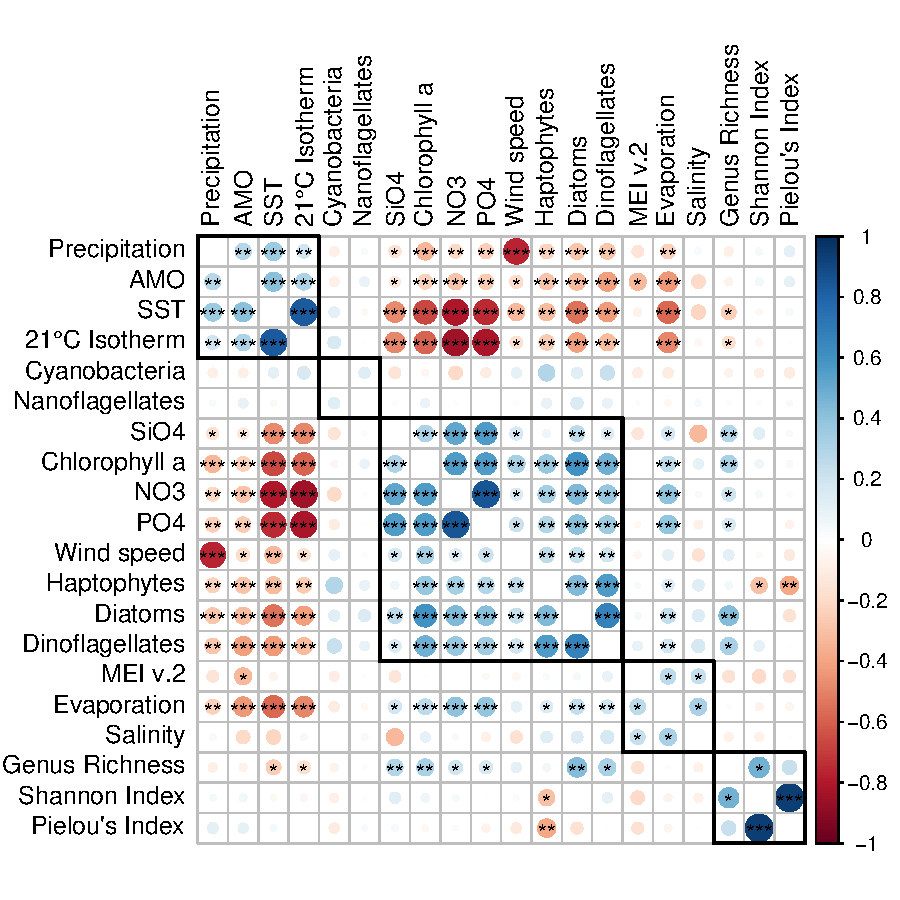
\includegraphics[width=\textwidth]{fig/CorrClustSupplementalPlot_v1.pdf}
\caption{Correlation matrix with clustering of environmental variables, diversity metrics and cell counts. Correlation was calcualted using a Spearman's rank correlation coefficient, the magnitude of the coefficient is indicated by the color of the circle. The size of the circle and significance level marking represents the calculated significance of the correlation deviating from 0 (p-value: ***\textless0.001, **\textless0.01, *\textless0.05). The time series were aditionally ordered by hierarchical clustering via the complete linkage method into 5 groups indicated by the black square border.}
\label{fig:sup:correlation}
\end{figure}



\section{Gradient Forest Analysis supplement}


\begin{figure}
\noindent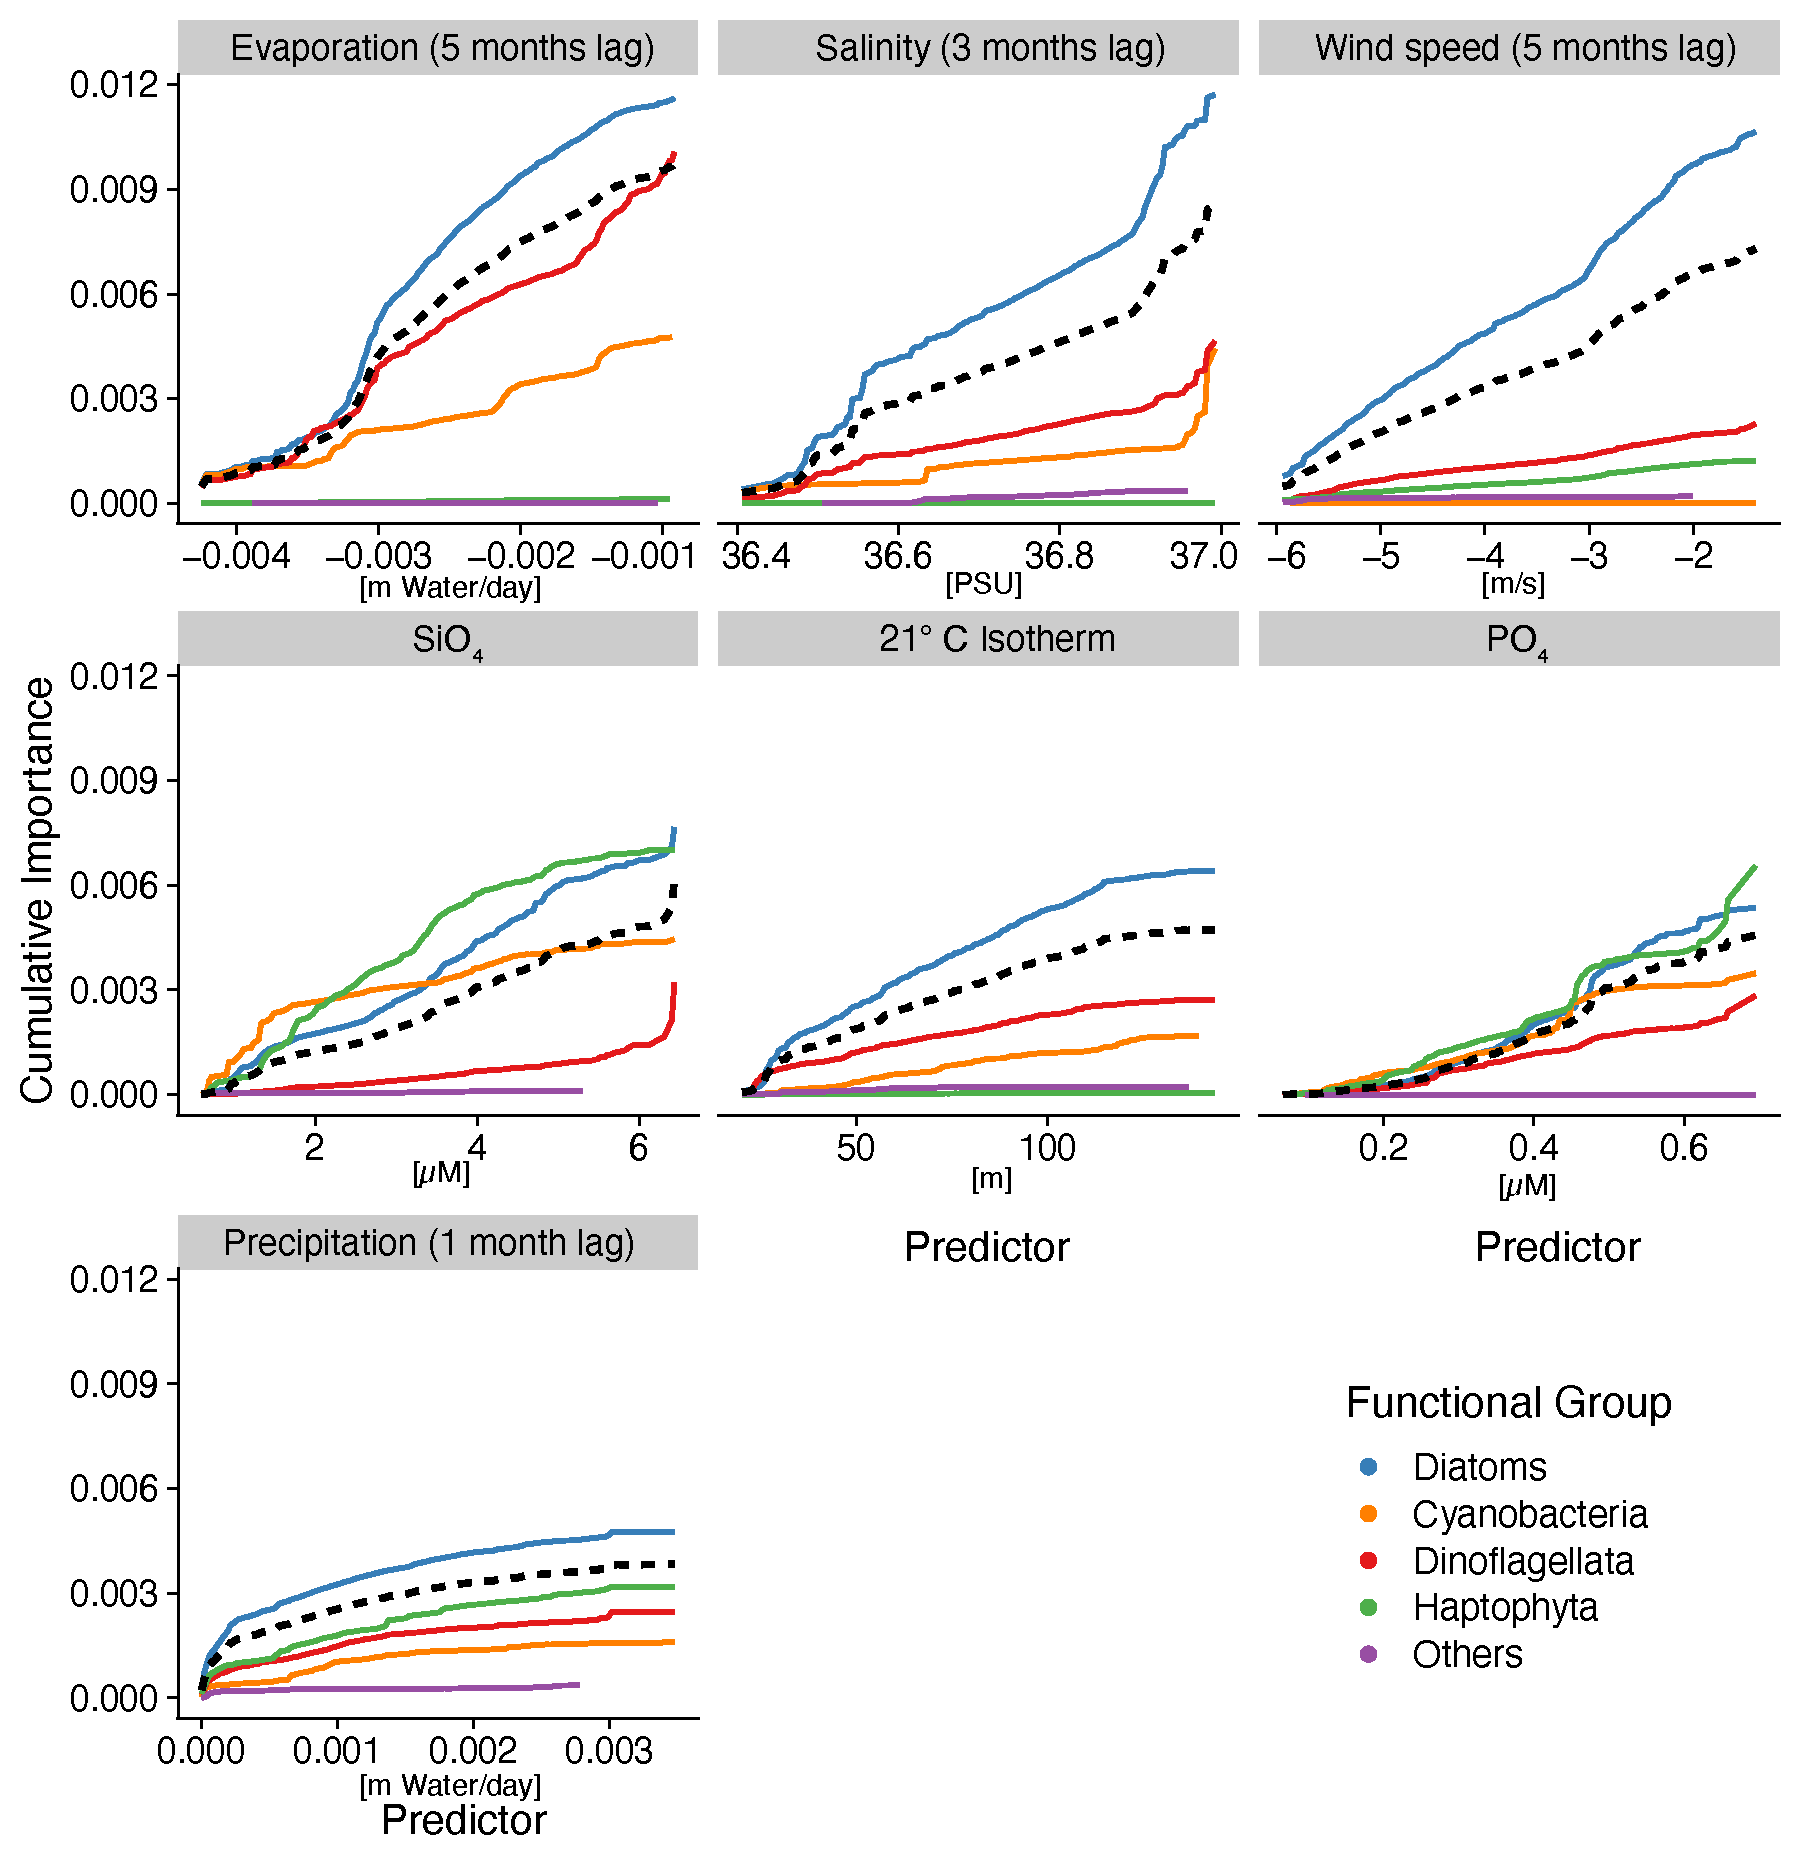
\includegraphics[width=\textwidth]{fig/FigureA2_GF_output_Supplement_v1.pdf}
\caption{Cumulative importance curves for all predictor variables not shown in the main figure. Dashed black line represents the cumulative importance across the entire community, colored lines represent functional groups. Gradient forest runs where done on Genus-level cell counts, integrated over the top 100 meters.}
\label{fig:sup:GFoutput_lags_extra}
\end{figure}


\begin{table}

\caption{Resulting $R^2$ weighted importance for running predictor variables together with time-lags to check if they provide a better fit to the data. Each column represents a single run, with resulting importance values for time series and monthly lags. The results were stable, so that repeated runs confirmed the chosen time lag. For in-situ variables,  we tested all measurements up to a lag of 3 months. For climate variables we tested up to a lag of 6 months and added a lag of 12 months for the climate indices. Time lag with maximum importance per variable are highlighted in bold and chosen for the final model run.}
\centering
\resizebox{\textwidth}{!}{\begin{tabular}[t]{rrrrrrrrrrrr}
\toprule
lag & NO3 & PO4 & SiO4 & SST & \qty{21}{\celsius} Isotherm & Salinity & AMO & MEI v.2 & Wind speed & Precipitation & Evaporation\\
\midrule
0 & \textbf{0.027} & \textbf{0.029} & \textbf{0.026} & \textbf{0.086} & \textbf{0.024} & 0.006 & 0.015 & 0.015 & 0.003 & 0.005 & 0.011\\
1 & 0.015 & 0.011 & 0.014 & 0.010 & 0.003 & 0.004 & 0.012 & 0.015 & 0.006 & \textbf{0.014} & 0.009\\
2 & 0.018 & 0.007 & 0.011 & 0.013 & 0.005 & 0.010 & \textbf{0.026} & 0.018 & 0.007 & 0.005 & 0.013\\
3 & 0.013 & 0.007 & 0.003 & 0.007 & 0.007 & \textbf{0.013} & 0.016 & 0.017 & 0.005 & 0.009 & 0.011\\
4 & NA & NA & NA & NA & NA & NA & 0.017 & \textbf{0.026} & 0.005 & 0.008 & 0.005\\
5 & NA & NA & NA & NA & NA & NA & 0.016 & 0.020 & \textbf{0.008} & 0.008 & \textbf{0.040}\\
6 & NA & NA & NA & NA & NA & NA & 0.017 & 0.012 & 0.005 & 0.006 & 0.004\\
\addlinespace
12 & NA & NA & NA & NA & NA & NA & 0.010 & 0.013 & NA & NA & NA\\
\bottomrule
\end{tabular}}
\label{tab:sup:GFlagtests}
\end{table}



\begin{figure}
\noindent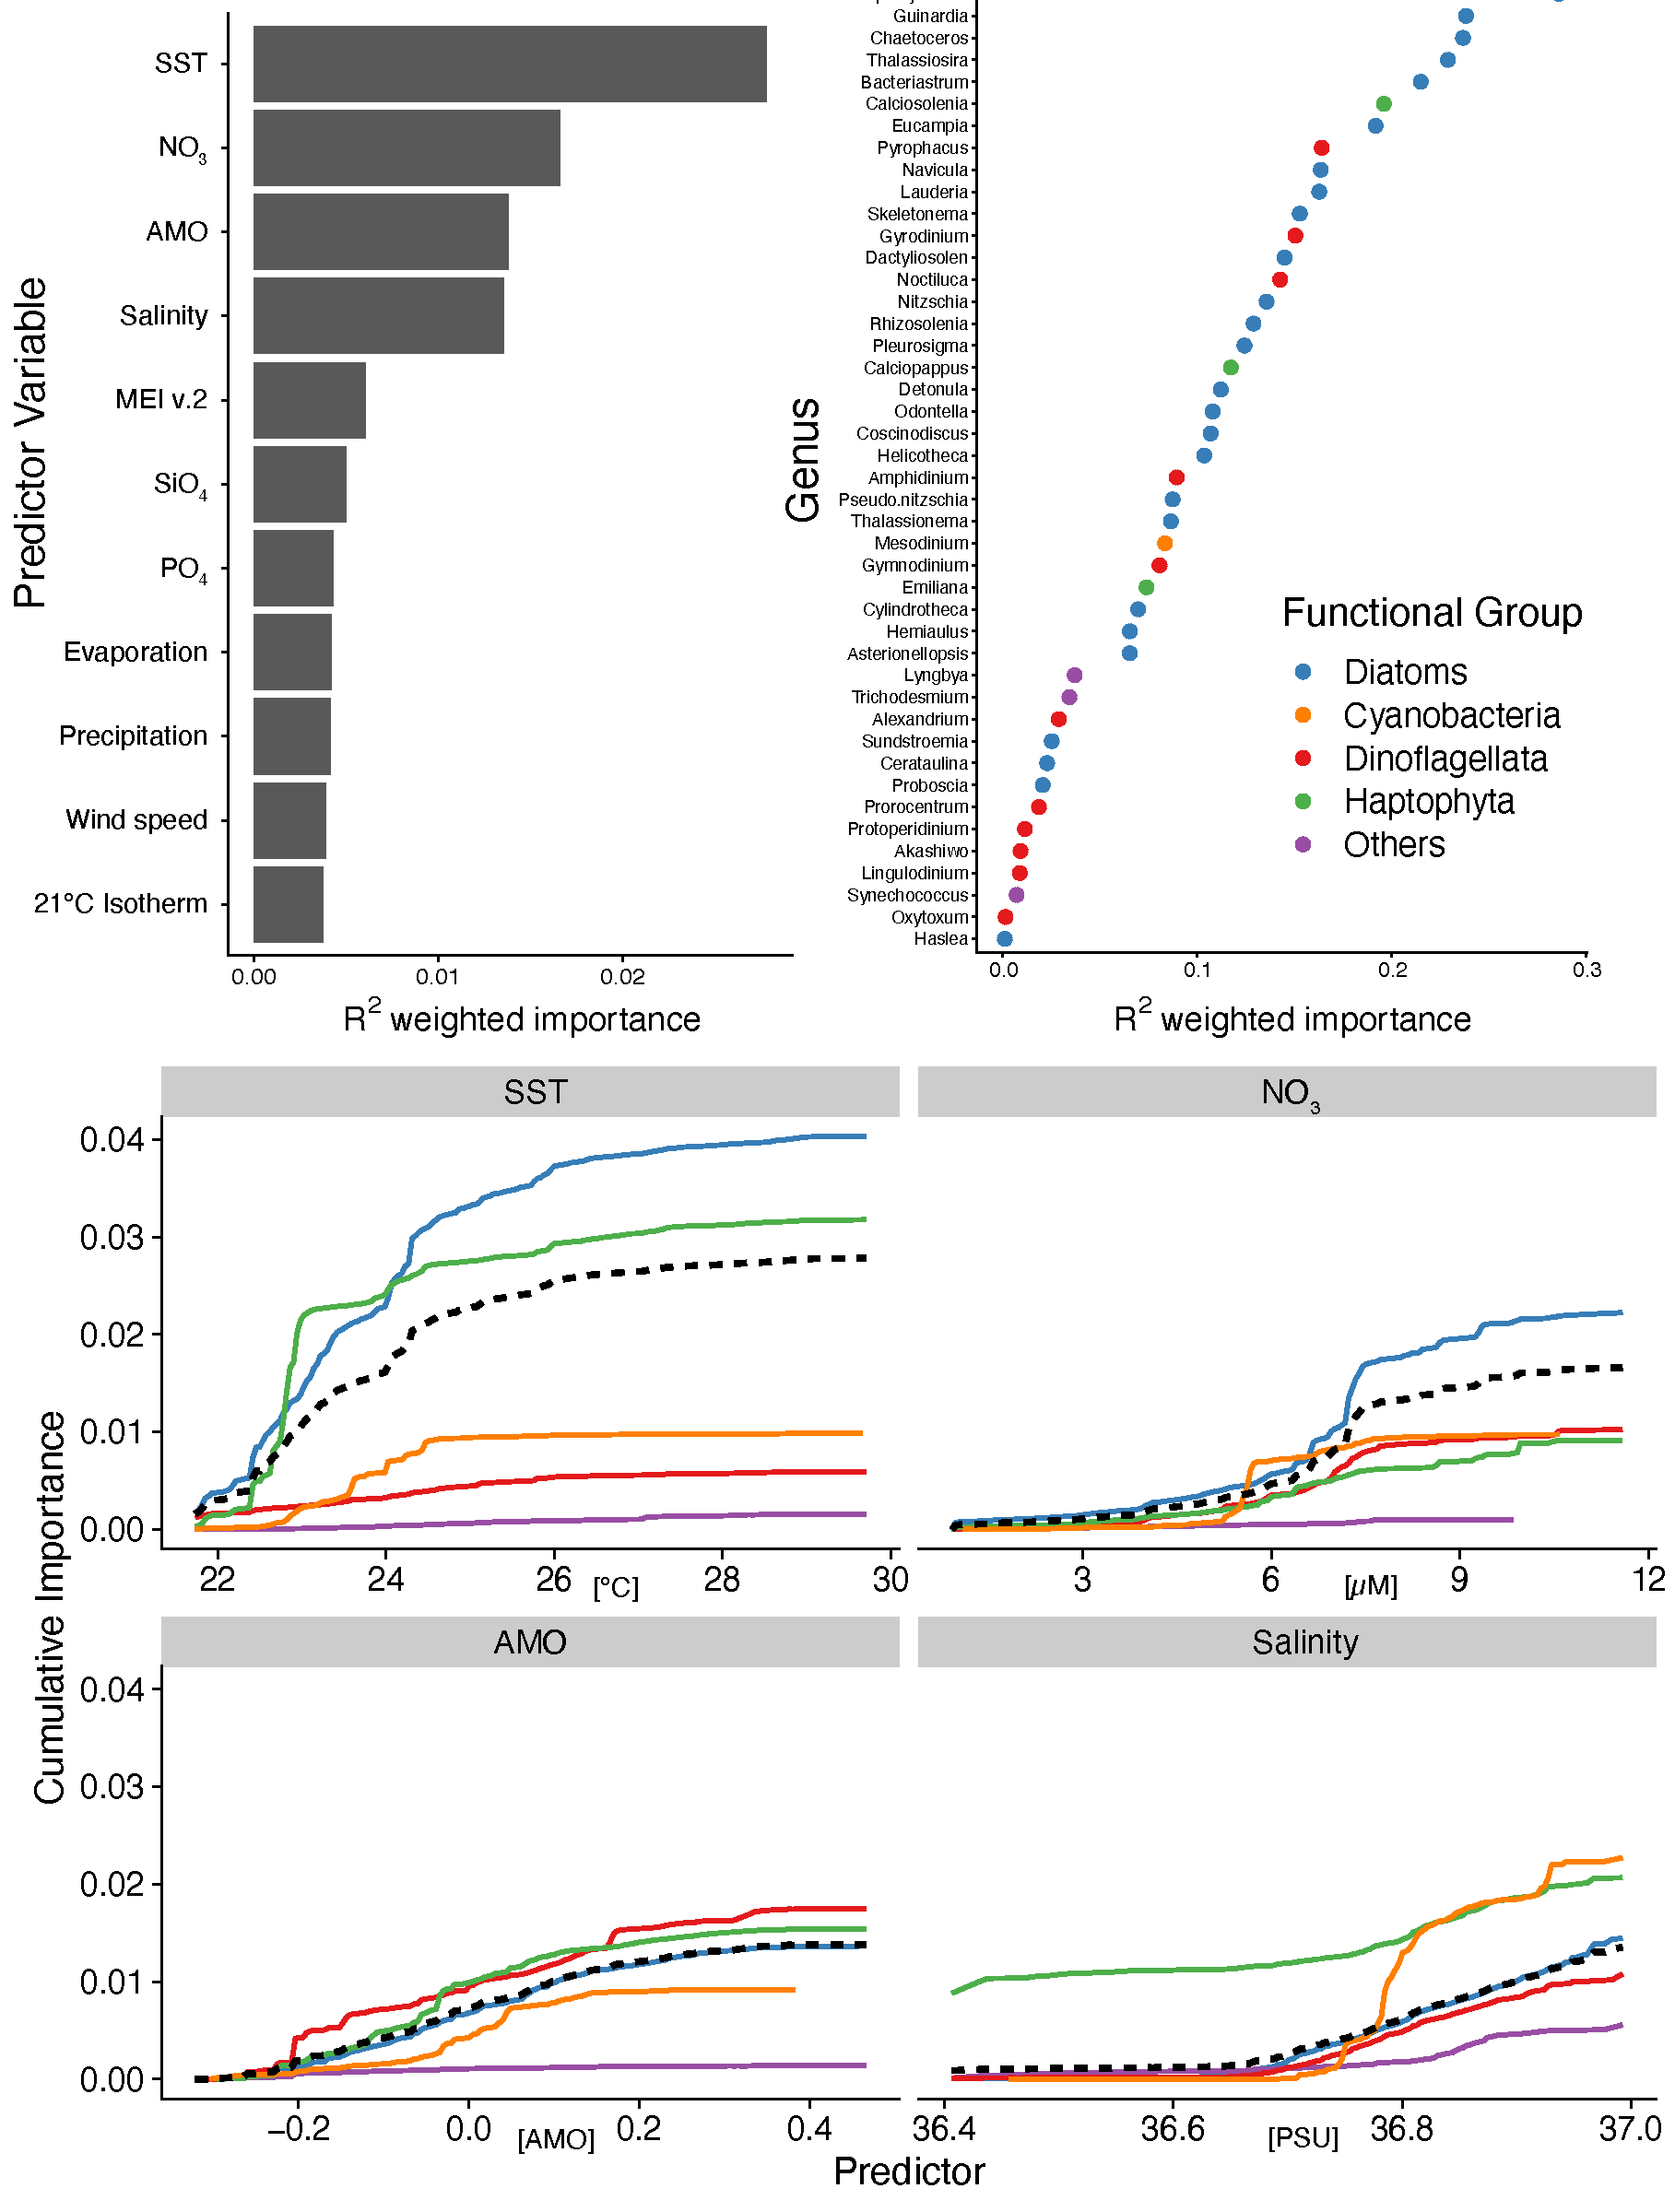
\includegraphics[width=\textwidth]{fig/FigureA3_GF_output_NOLAG_v1.pdf}
\caption{Gradient Forest analysis of monthly community data at a genus level. (a) Predictor variables ranked according to overall weighted importance in predicting shifts in abundances. (b) Phytoplankton genera that could be predicted ranked according to the predictive power via the weighted importance. (c) Cumulative importance curves for the predictor variables. Black line shows cumulative importance across predictor range for the entire model and all genera. Dashed colored lines represent the responses of individual functional groups.}
\label{fig:sup:GFoutput_nolags}
\end{figure}


\begin{figure}
\noindent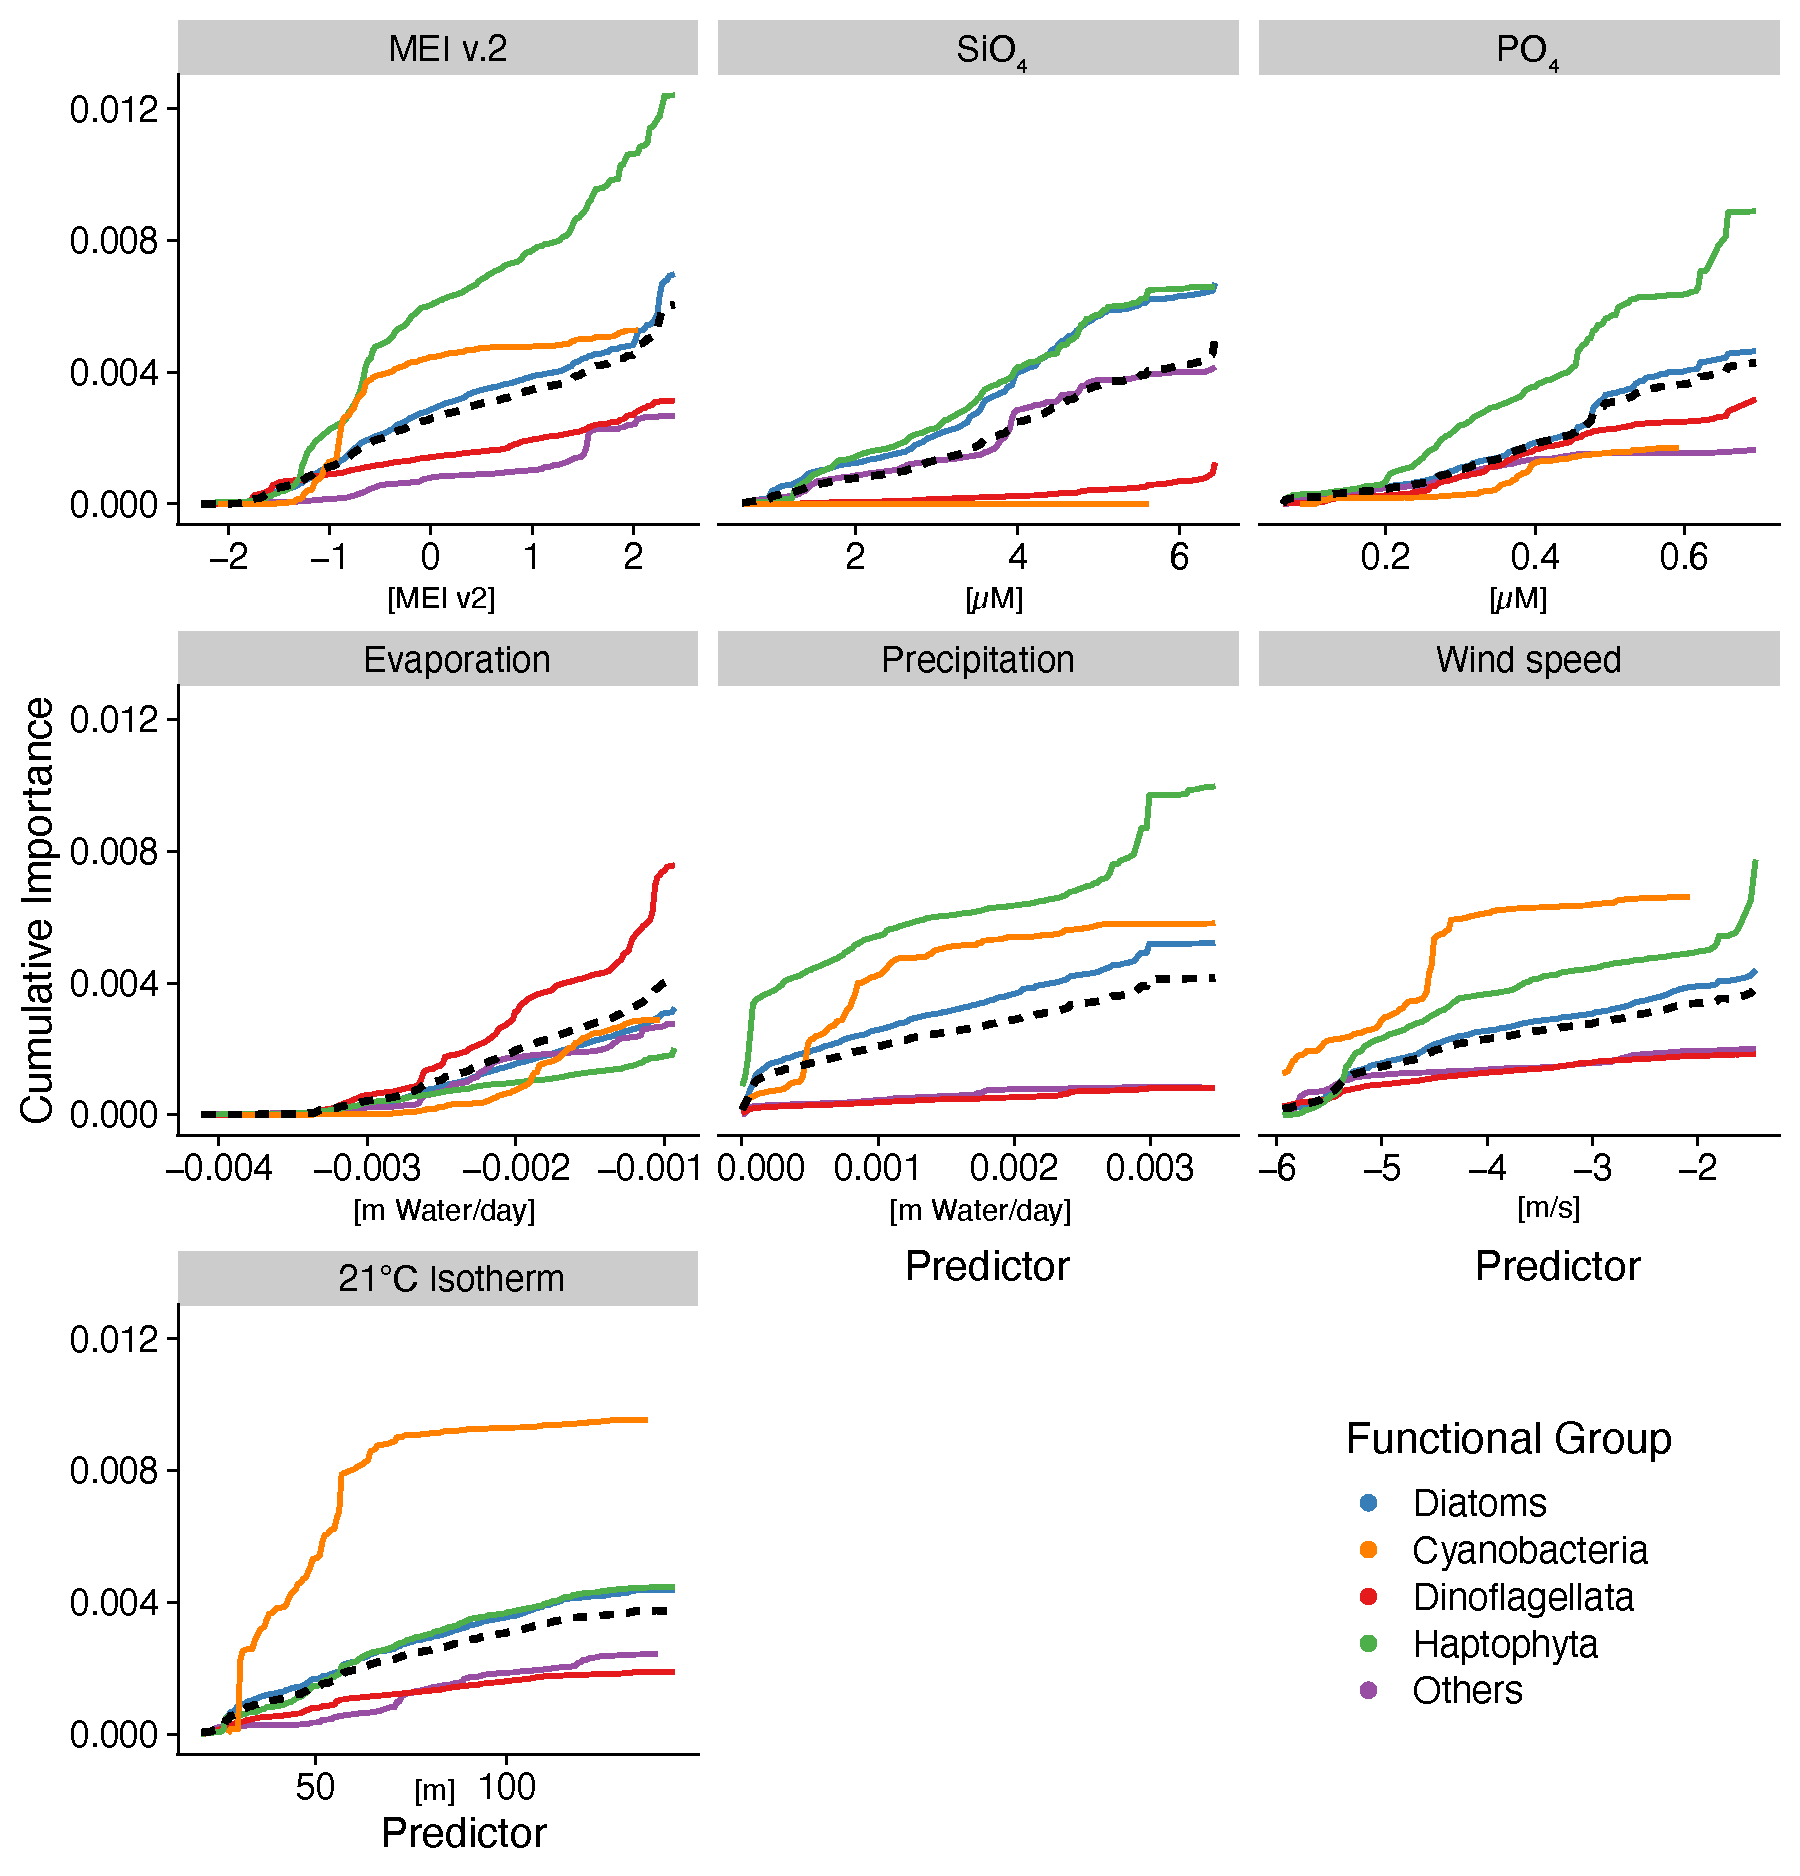
\includegraphics[width=\textwidth]{fig/FigureA4_GF_output_Supplement_NOLAG_v1.pdf}
\caption{Cumulative importance curves for all variables not shown in the previous figure. Dashed black line represents the cumulative importance across the entire community, colored lines represent functional groups. Gradient forest runs where done on Genus-level cell counts, integrated over the top 100 meters.}
\label{fig:sup:GFoutput_nolags_extra}
\end{figure}



%%%%%%%%%%%%%%%%%%%%%%%%%%%%%%%%%%%%%%%%%%%%%%%
% Optional Glossary, Notation or Acronym section goes here:
%
% Glossary is only allowed in Reviews of Geophysics
%  \begin{glossary}
%  \term{Term}
%   Term Definition here
%  \term{Term}
%   Term Definition here
%  \term{Term}
%   Term Definition here
%  \end{glossary}


%%%%%%%%%%%%%%%%%%%%%%%%%%%%%%%%%%%%%%%%%%%%%%%
% Acronyms
%% NOTE that acronyms in the final published version will be spelled out when used in figure captions.
%   \begin{acronyms}
%   \acro{Acronym}
%   Definition here
%   \acro{EMOS}
%   Ensemble model output statistics
%   \acro{ECMWF}
%   Centre for Medium-Range Weather Forecasts
%   \end{acronyms}


%%%%%%%%%%%%%%%%%%%%%%%%%%%%%%%%%%%%%%%%%%%%%%%
% Notation
%   \begin{notation}
%   \notation{$a+b$} Notation Definition here
%   \notation{$e=mc^2$}
%   Equation in German-born physicist Albert Einstein's theory of special
%  relativity that showed that the increased relativistic mass ($m$) of a
%  body comes from the energy of motion of the body—that is, its kinetic
%  energy ($E$)—divided by the speed of light squared ($c^2$).
%   \end{notation}




%%%%%%%%%%%%%%%%%%%%%%%%%%%%%%%%%%%%%%%%%%%%%%%
%
% DATA SECTION and ACKNOWLEDGMENTS
%
%%%%%%%%%%%%%%%%%%%%%%%%%%%%%%%%%%%%%%%%%%%%%%%

%!
\section*{Open Research Section}
This section MUST contain a statement that describes where the data supporting the conclusions can be obtained. Data cannot be listed as ''Available from authors'' or stored solely in supporting information. Citations to archived data should be included in your reference list. Wiley will publish it as a separate section on the paper’s page. Examples and complete information are here:
https://www.agu.org/Publish with AGU/Publish/Author Resources/Data for Authors

\section*{As Applicable – Inclusion in Global Research Statement}
The Authorship: Inclusion in Global Research policy aims to promote greater equity and transparency in research collaborations. AGU Publications encourage research collaborations between regions, countries, and communities and expect authors to include their local collaborators as co-authors when they meet the AGU Publications authorship criteria (described here: https://www.agu.org/publications/authors/policies\#authorship). Those who do not meet the criteria should be included in the Acknowledgement section. We encourage researchers to consider recommendations from The TRUST CODE - A Global Code of Conduct for Equitable Research Partnerships (https://www.globalcodeofconduct.org/) when conducting and reporting their research, as applicable, and encourage authors to include a disclosure statement pertaining to the ethical and scientific considerations of their research collaborations in an “Inclusion in Global Research Statement’ as a standalone section in the manuscript following the Conclusions section. This can include disclosure of permits, authorizations, permissions and/or any formal agreements with local communities or other authorities, additional acknowledgements of local help received, and/or description of end-users of the research. You can learn more about the policy in this editorial. Example statements can be found in the following published papers: 
%Holt et al. (https://agupubs.onlinelibrary.wiley.com/doi/full/10.1029/2022JG007188), 
%Sánchez-Gutiérrez et al. (https://agupubs.onlinelibrary.wiley.com/doi/abs/10.1029/2023JG007554), 
%Tully et al. (https://agupubs.onlinelibrary.wiley.com/doi/epdf/10.1029/2022JG007128) 
%Please note that these statements are titled as “Global Research Collaboration Statements” from a previous pilot requirement in JGR Biogeosciences. The pilot has ended and statements should now be titled “Inclusion in Global Research Statement”.


%!
\acknowledgments
Thank you to all who have helped, communicated, provided data. Claudia Benitez-Nelson, Digna Rueda-Roa, James Pinckney.

%Enter acknowledgments here. This section is to acknowledge funding, thank colleagues, enter any secondary affiliations, and so on.


%%%%%%%%%%%%%%%%%%%%%%%%%%%%%%%%%%%%%%%%%%%%%%%
% REFERENCES and BIBLIOGRAPHY
%
%\bibliography{<name of your .bib file>} don't specify the file extension
% don't specify bibliographystyle
%
%%%%%%%%%%%%%%%%%%%%%%%%%%%%%%%%%%%%%%%%%%%%%%%

\bibliography{references}



%Reference citation instructions and examples:
%
% Please use ONLY \cite and \citeA for reference citations.
% \cite for parenthetical references
% ...as shown in recent studies (Simpson et al., 2019)
% \citeA for in-text citations
% ...Simpson et al. (2019) have shown...
%
%
%...as shown by \citeA{jskilby}.
%...as shown by \citeA{lewin76}, \citeA{carson86}, \citeA{bartoldy02}, and \citeA{rinaldi03}.
%...has been shown \cite{jskilbye}.
%...has been shown \cite{lewin76,carson86,bartoldy02,rinaldi03}.
%... \cite <i.e.>[]{lewin76,carson86,bartoldy02,rinaldi03}.
%...has been shown by \cite <e.g.,>[and others]{lewin76}.
%
% apacite uses < > for prenotes and [ ] for postnotes
% DO NOT use other cite commands (e.g., \citet, \citep, \citeyear, \nocite, \citealp, etc.).
%




\end{document}



More Information and Advice:

%%%%%%%%%%%%%%%%%%%%%%%%%%%%%%%%%%%%%%%%%%%%%%%
%
%  SECTION HEADS
%
%%%%%%%%%%%%%%%%%%%%%%%%%%%%%%%%%%%%%%%%%%%%%%%

% Capitalize the first letter of each word (except for
% prepositions, conjunctions, and articles that are
% three or fewer letters).

% AGU follows standard outline style; therefore, there cannot be a section 1 without
% a section 2, or a section 2.3.1 without a section 2.3.2.
% Please make sure your section numbers are balanced.
% ---------------
% Level 1 head
%
% Use the \section{} command to identify level 1 heads;
% type the appropriate head wording between the curly
% brackets, as shown below.
%
%An example:
%\section{Level 1 Head: Introduction}
%
% ---------------
% Level 2 head
%
% Use the \subsection{} command to identify level 2 heads.
%An example:
%\subsection{Level 2 Head}
%
% ---------------
% Level 3 head
%
% Use the \subsubsection{} command to identify level 3 heads
%An example:
%\subsubsection{Level 3 Head}
%
%---------------
% Level 4 head
%
% Use the \subsubsubsection{} command to identify level 3 heads
% An example:
%\subsubsubsection{Level 4 Head} An example.
%
%%%%%%%%%%%%%%%%%%%%%%%%%%%%%%%%%%%%%%%%%%%%%%%
%
%  IN-TEXT LISTS
%
%%%%%%%%%%%%%%%%%%%%%%%%%%%%%%%%%%%%%%%%%%%%%%%
%
% Do not use bulleted lists; enumerated lists are okay.
% \begin{enumerate}
% \item
% \item
% \item
% \end{enumerate}
%
%%%%%%%%%%%%%%%%%%%%%%%%%%%%%%%%%%%%%%%%%%%%%%%
%
%  EQUATIONS
%
%%%%%%%%%%%%%%%%%%%%%%%%%%%%%%%%%%%%%%%%%%%%%%%

% Single-line equations are centered.
% Equation arrays will appear left-aligned.

Math coded inside display math mode \[ ...\]
 will not be numbered, e.g.,:
 \[ x^2=y^2 + z^2\]

 Math coded inside \begin{equation} and \end{equation} will
 be automatically numbered, e.g.,:
 \begin{equation}
 x^2=y^2 + z^2
 \end{equation}


% To create multiline equations, use the
% \begin{eqnarray} and \end{eqnarray} environment
% as demonstrated below.
\begin{eqnarray}
  x_{1} & = & (x - x_{0}) \cos \Theta \nonumber \\
        && + (y - y_{0}) \sin \Theta  \nonumber \\
  y_{1} & = & -(x - x_{0}) \sin \Theta \nonumber \\
        && + (y - y_{0}) \cos \Theta.
\end{eqnarray}

%If you don't want an equation number, use the star form:
%\begin{eqnarray*}...\end{eqnarray*}

% Break each line at a sign of operation
% (+, -, etc.) if possible, with the sign of operation
% on the new line.

% Indent second and subsequent lines to align with
% the first character following the equal sign on the
% first line.

% Use an \hspace{} command to insert horizontal space
% into your equation if necessary. Place an appropriate
% unit of measure between the curly braces, e.g.
% \hspace{1in}; you may have to experiment to achieve
% the correct amount of space.


%%%%%%%%%%%%%%%%%%%%%%%%%%%%%%%%%%%%%%%%%%%%%%%
%
%  EQUATION NUMBERING: COUNTER
%
%%%%%%%%%%%%%%%%%%%%%%%%%%%%%%%%%%%%%%%%%%%%%%%

% You may change equation numbering by resetting
% the equation counter or by explicitly numbering
% an equation.

% To explicitly number an equation, type \eqnum{}
% (with the desired number between the brackets)
% after the \begin{equation} or \begin{eqnarray}
% command.  The \eqnum{} command will affect only
% the equation it appears with; LaTeX will number
% any equations appearing later in the manuscript
% according to the equation counter.
%

% If you have a multiline equation that needs only
% one equation number, use a \nonumber command in
% front of the double backslashes (\\) as shown in
% the multiline equation above.

% If you are using line numbers, remember to surround
% equations with \begin{linenomath*}...\end{linenomath*}

%  To add line numbers to lines in equations:
%  \begin{linenomath*}
%  \begin{equation}
%  \end{equation}
%  \end{linenomath*}



